\section{Landing Page}
\begin{figure}[H]
    \centering
    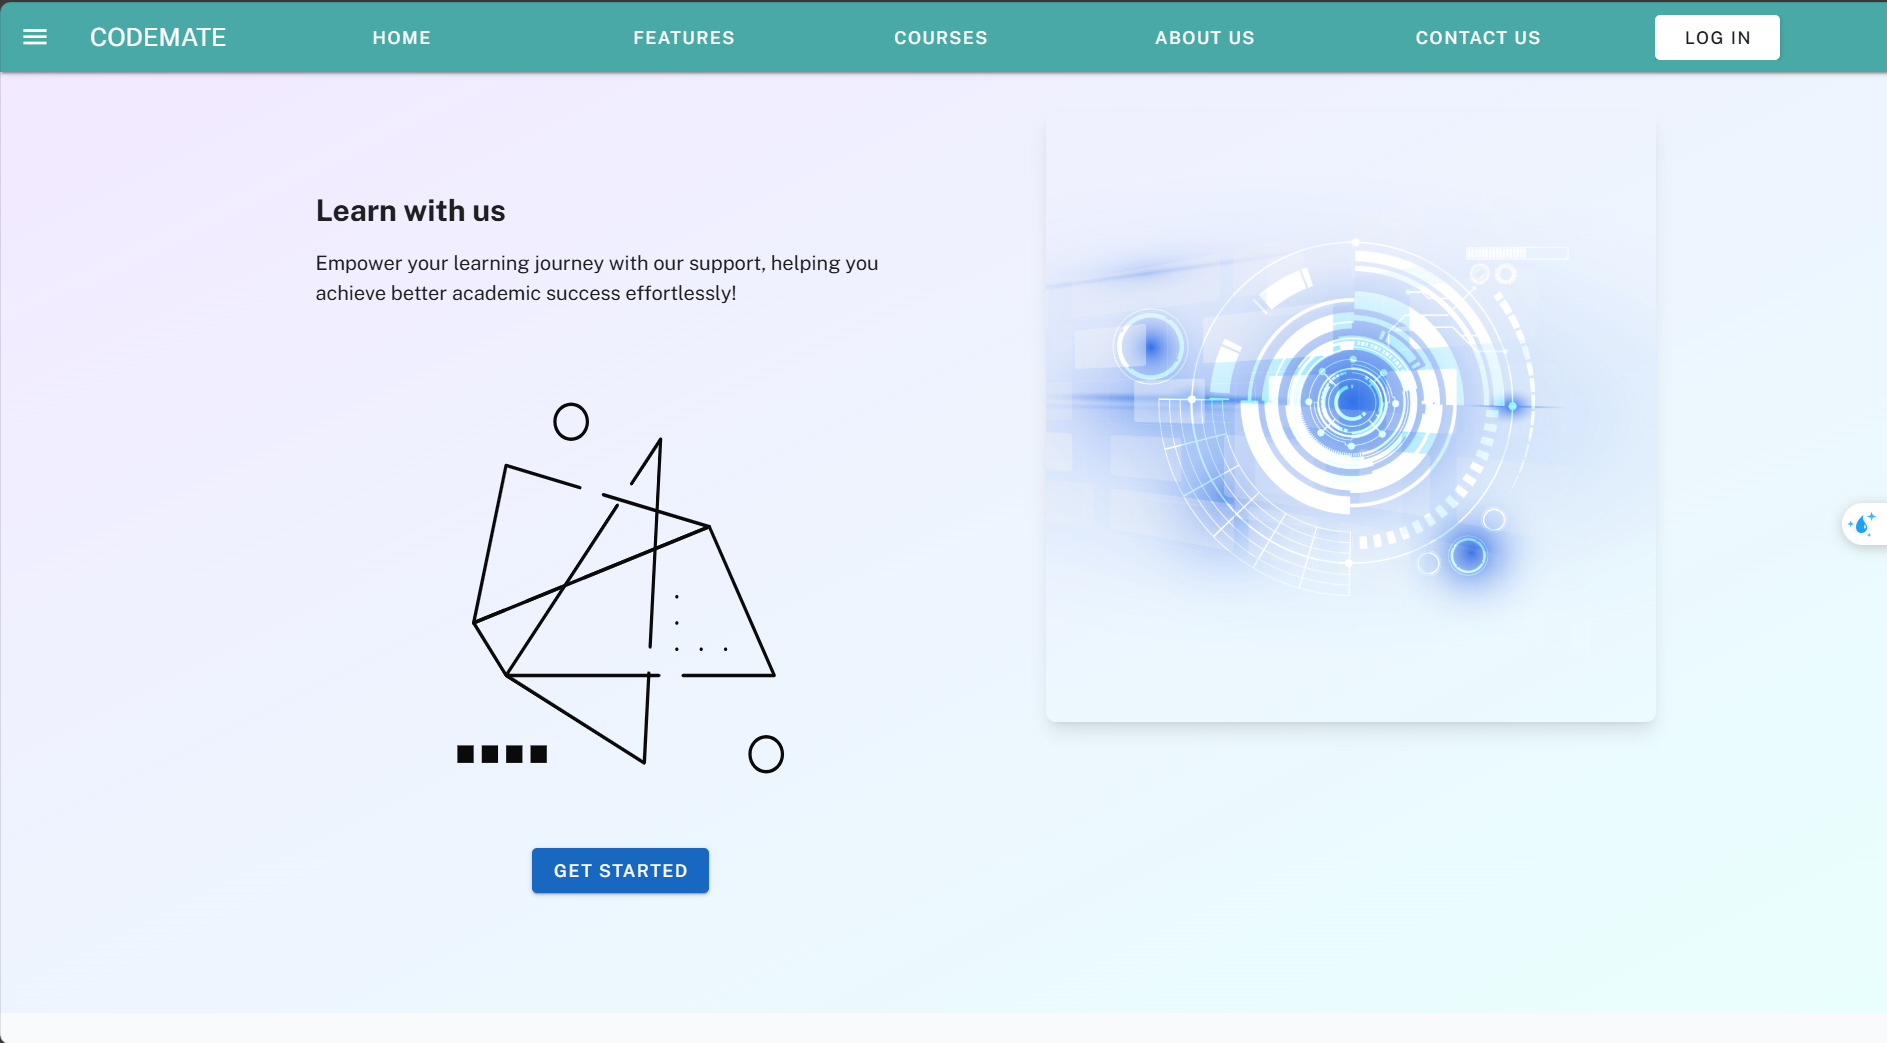
\includegraphics[width=0.8\textwidth]{images/CapScreen_Student/LandingPage.png}
    \caption{Giao diện trang chủ của hệ thống}
    \label{fig:landing_page}
\end{figure}
Đây là giao diện trang chủ của hệ thống, nơi người dùng có thể tìm hiểu về các chức năng chính của hệ thống và đăng nhập vào tài khoản cá nhân. Giao diện được thiết kế đơn giản, dễ sử dụng và thân thiện với người dùng.
\section{Đăng nhập}
\begin{figure}[H]
    \centering
    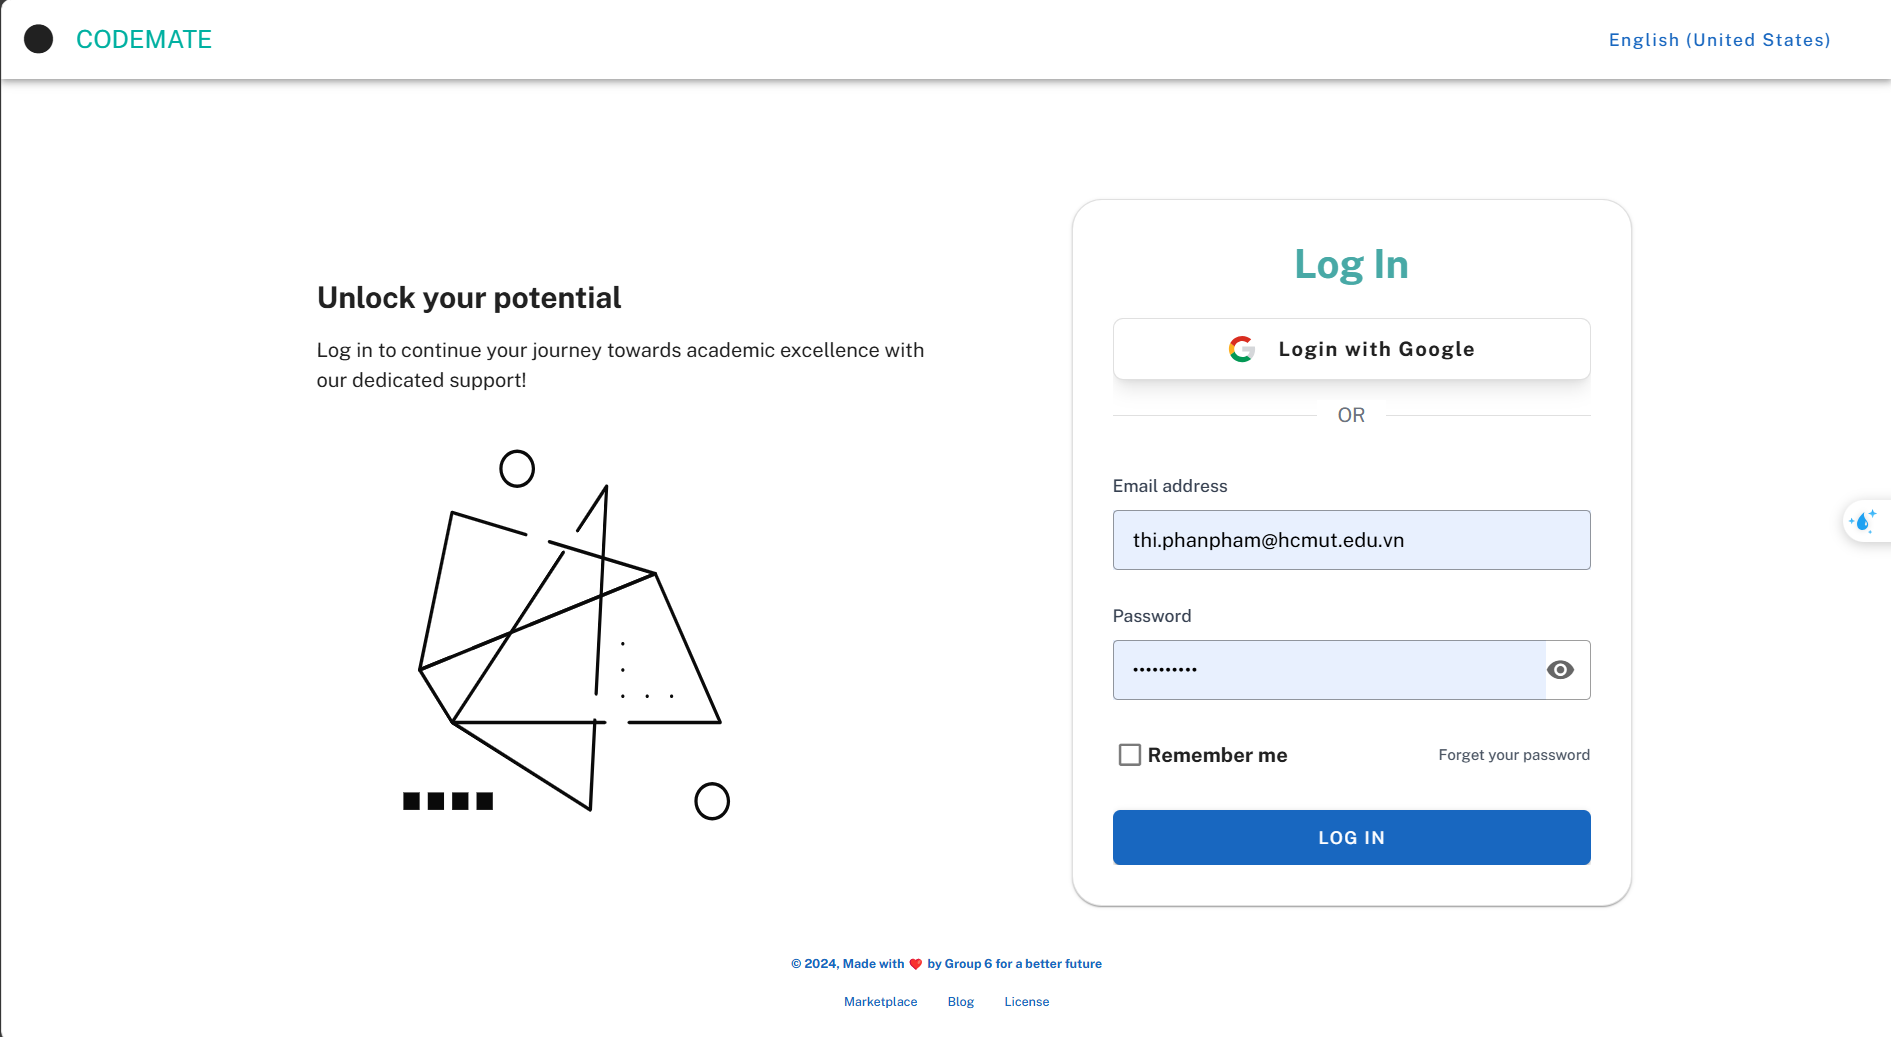
\includegraphics[width=0.8\textwidth]{images/CapScreen_Student/Login.png}
    \caption{Giao diện đăng nhập của hệ thống}
    \label{fig:login_page}
\end{figure}
Giao diện đăng nhập cho phép người dùng đăng nhập vào tài khoản cá nhân bằng email và mật khẩu hoặc thông qua tài khoản Google. Hệ thống hỗ trợ xác thực người dùng và phân quyền theo vai trò (học viên, giảng viên, quản trị viên).
\section{Profile}
\begin{figure}[H]
    \centering
    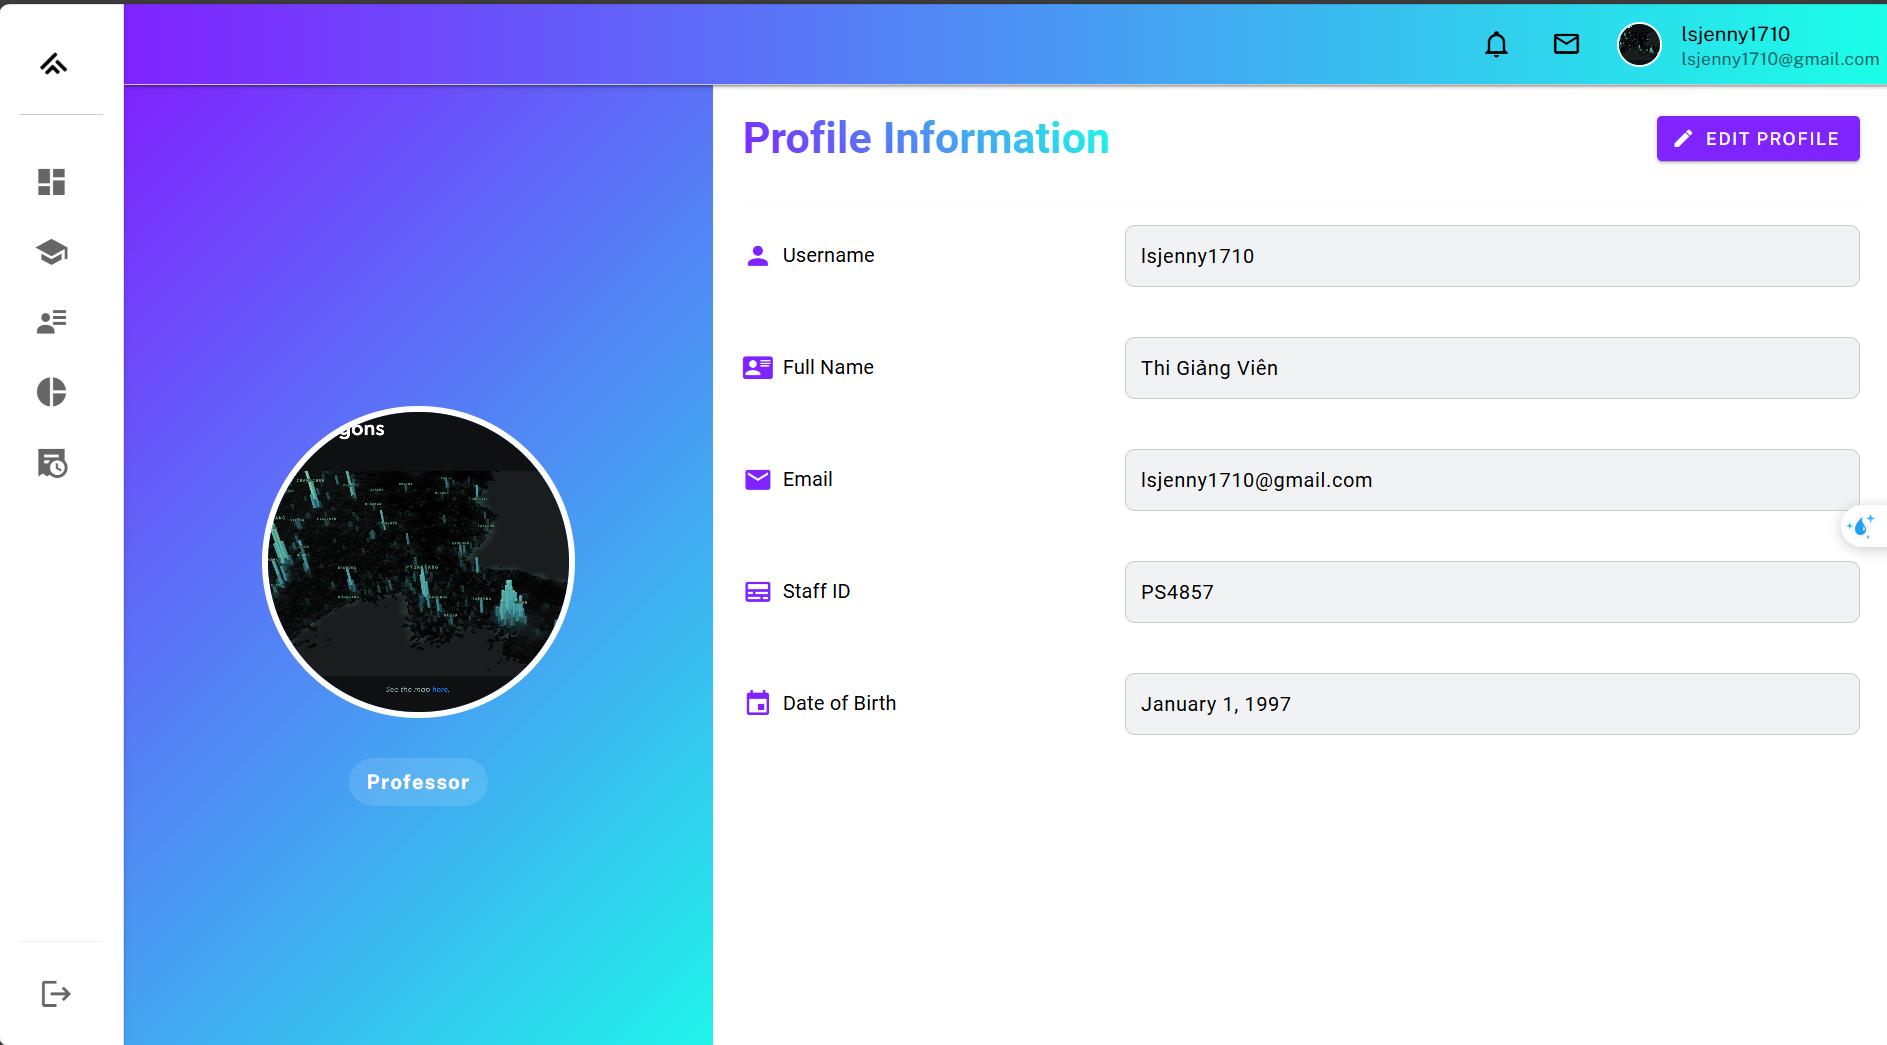
\includegraphics[width=0.8\textwidth]{images/CapScreen_Student/Profile.png}
    \caption{Giao diện thông tin cá nhân của sinh viên}
    \label{fig:profile_page}
\end{figure}
Giao diện thông tin cá nhân cho phép người dùng xem và chỉnh sửa thông tin cá nhân của mình, bao gồm tên, email, số điện thoại và ảnh đại diện.
\section{Sinh viên}
\subsection{Giao diện chính}
\begin{figure}[H]
    \centering
    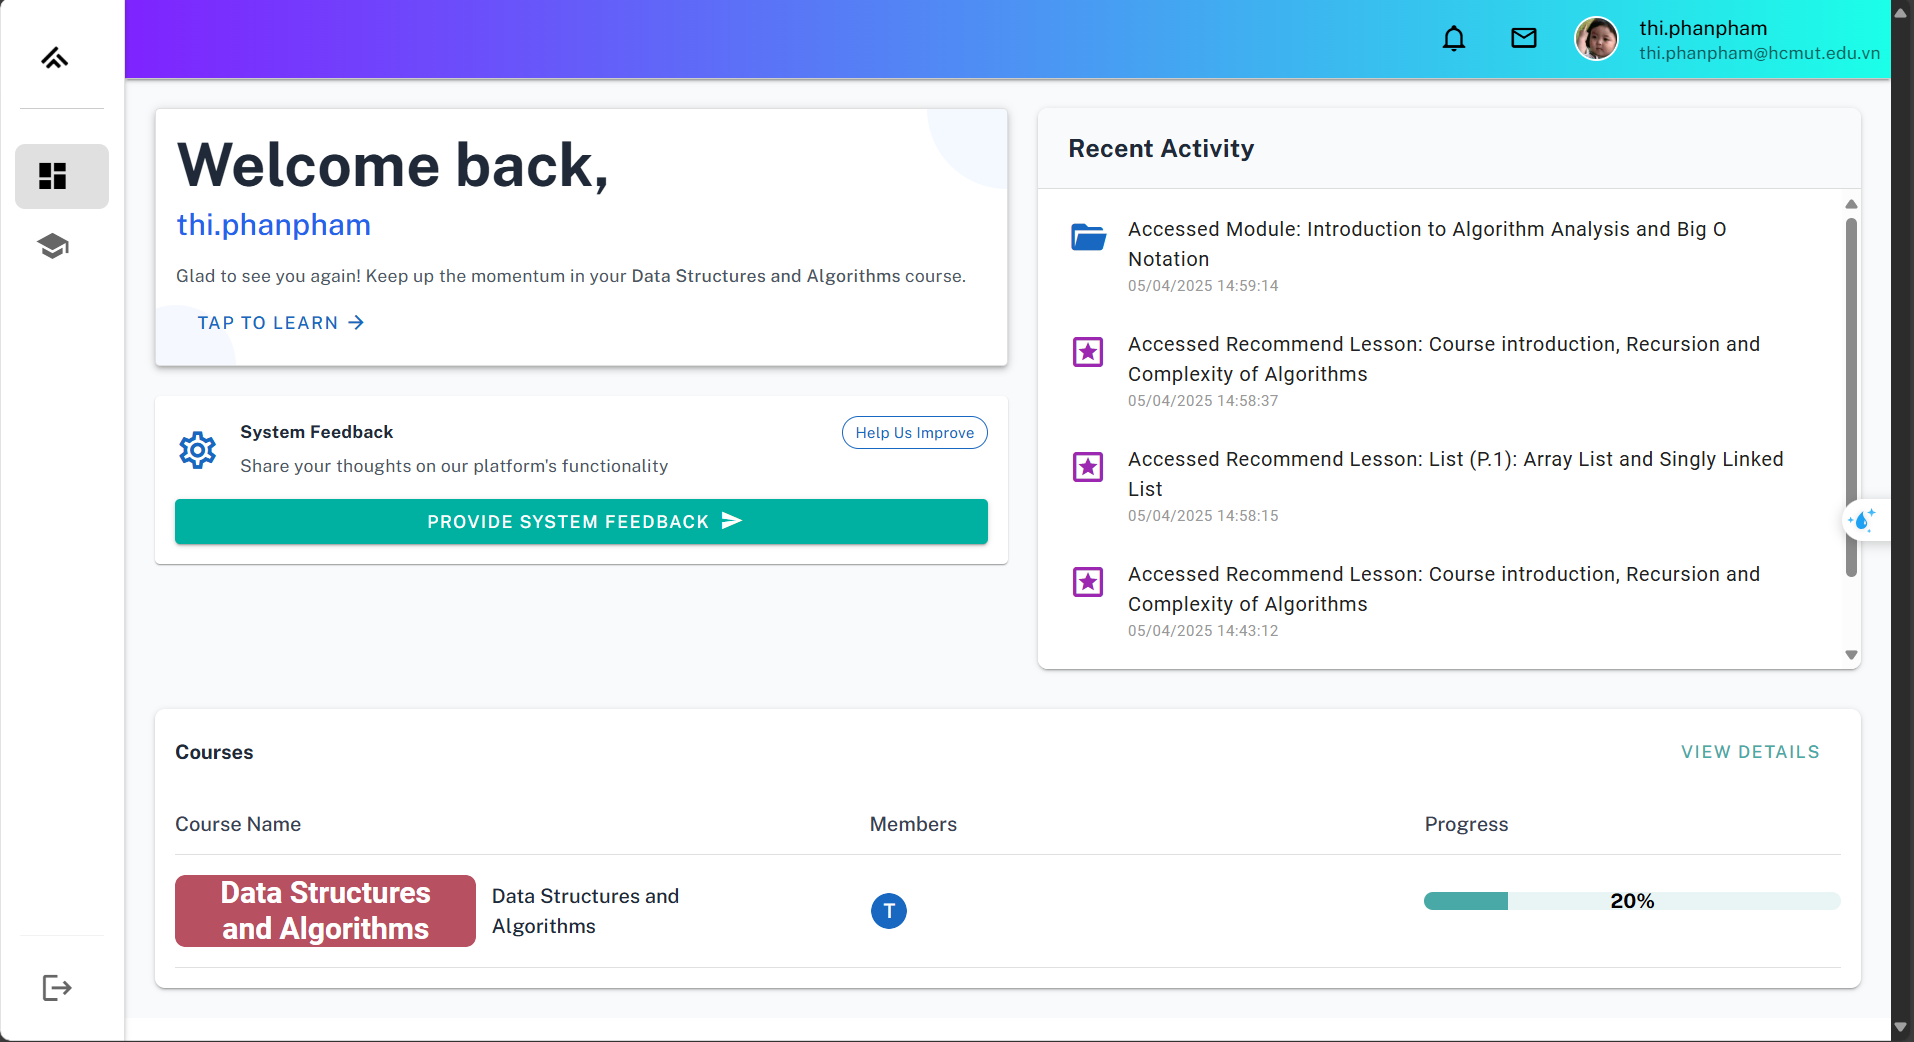
\includegraphics[width=0.8\textwidth]{images/CapScreen_Student/Dashboard.png}
    \caption{Giao diện chính của sinh viên}
    \label{fig:home_page}
\end{figure}
Giao diện chính của sinh viên hiển thị danh sách các khóa học mà sinh viên đang theo học. Tại đây, sinh viên có thể xem thông tin khóa học, bài học và bài tập cần hoàn thành. Ngoài ra sinh viên có thể xem các hoạt động gần đây của mình và gửi feedback cho hệ thống nếu có vấn đề gì.
\subsection{Quản lý khóa học}
\begin{figure}[H]
    \centering
    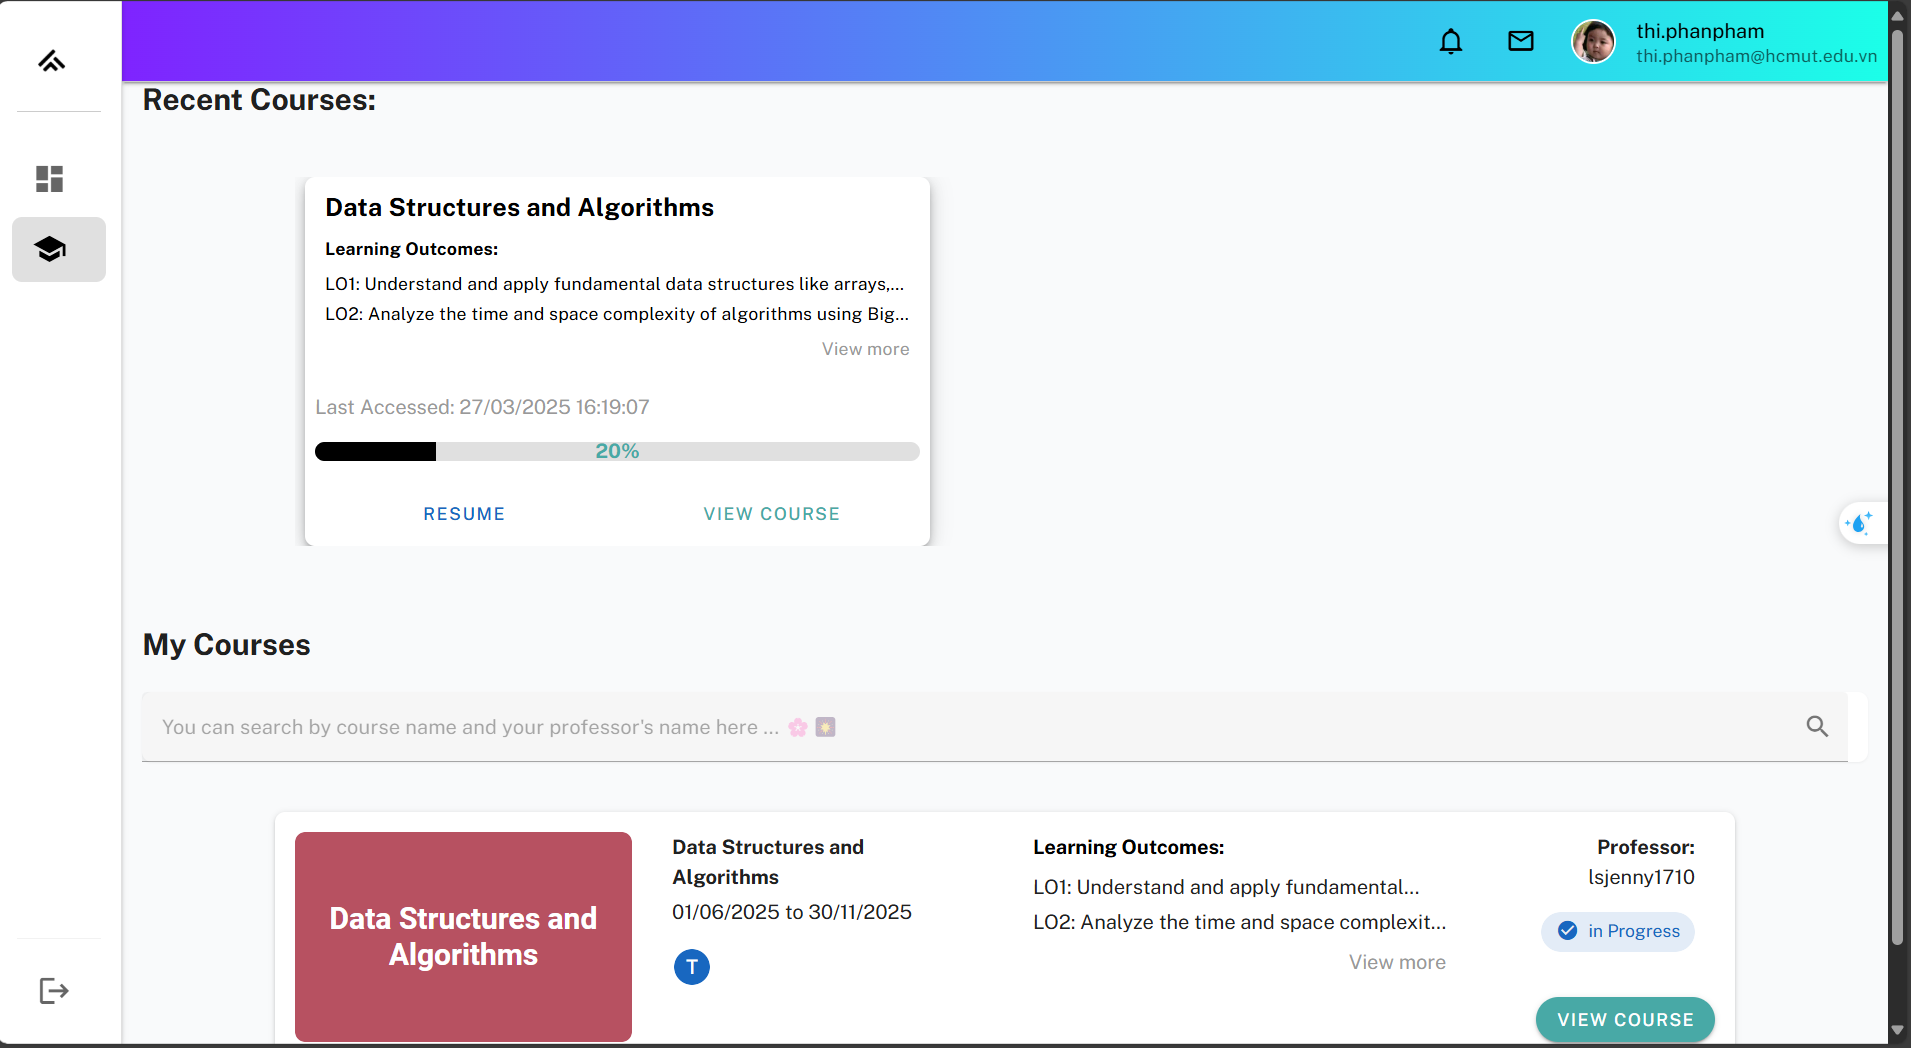
\includegraphics[width=0.8\textwidth]{images/CapScreen_Student/CoursesList.png}
    \caption{Giao diện quản lý khóa học của sinh viên}
    \label{fig:course_page}
\end{figure}
Giao diện quản lý khóa học cho phép sinh viên xem danh sách các khóa học mà mình đang theo học. Tại đây, sinh viên có thể xem thông tin chi tiết về khóa học, bao gồm tên khóa học, giảng viên phụ trách, thời gian bắt đầu và kết thúc, Learning Outcomes và trạng thái hoàn thành của khóa học.
\subsection{Chi tiết khóa học}
\begin{figure}[H]
    \centering
    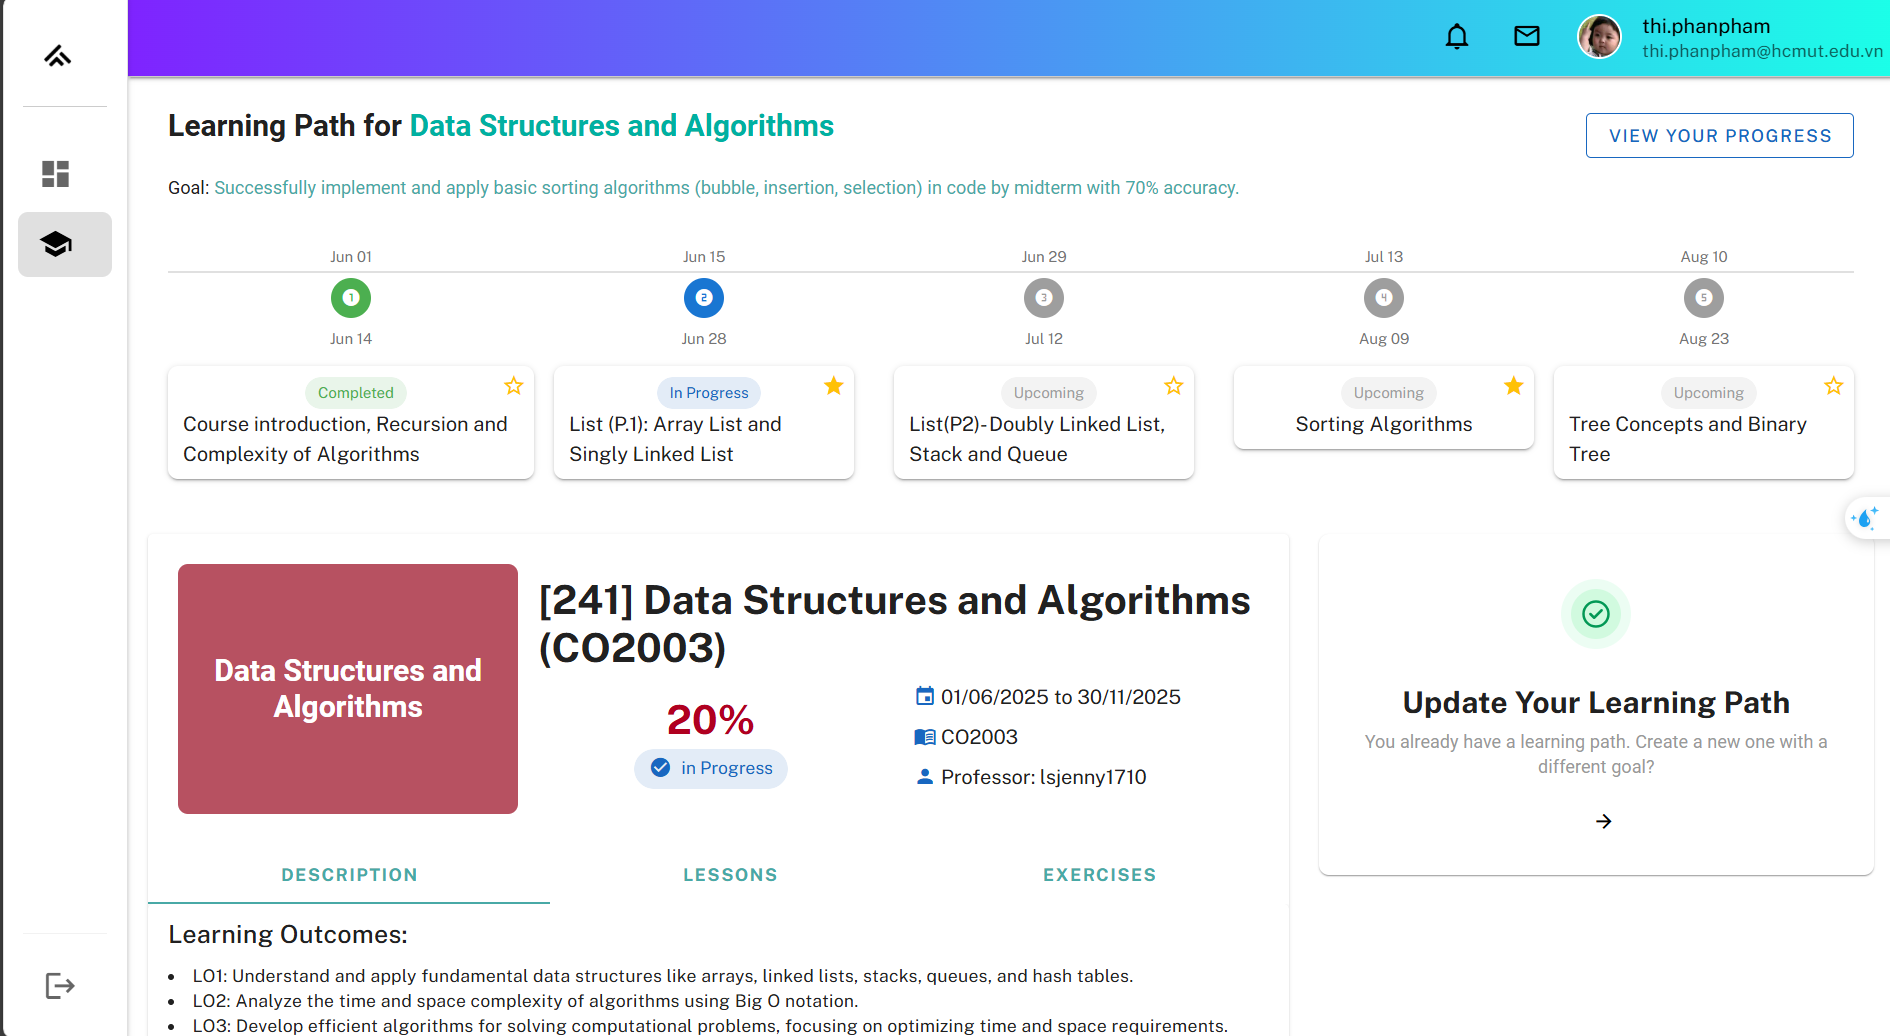
\includegraphics[width=0.8\textwidth]{images/CapScreen_Student/CoursesDetail.png}
    \caption{Giao diện chi tiết khóa học của sinh viên}
    \label{fig:course_detail_page}
\end{figure}
Giao diện chi tiết khóa học cho phép sinh viên xem thông tin chi tiết về khóa học, bao gồm danh sách bài học, bài tập và tiến độ học tập. Tại đây, sinh viên có thể xem các bài học đã hoàn thành và chưa hoàn thành, cũng như các bài tập cần làm. Ngoài ra, nếu sinh viên đã sinh lộ trình học thì có thể xem lộ trình học của mình tại đây.
\subsection{Chi tiết bài học}
\begin{figure}[H]
    \centering
    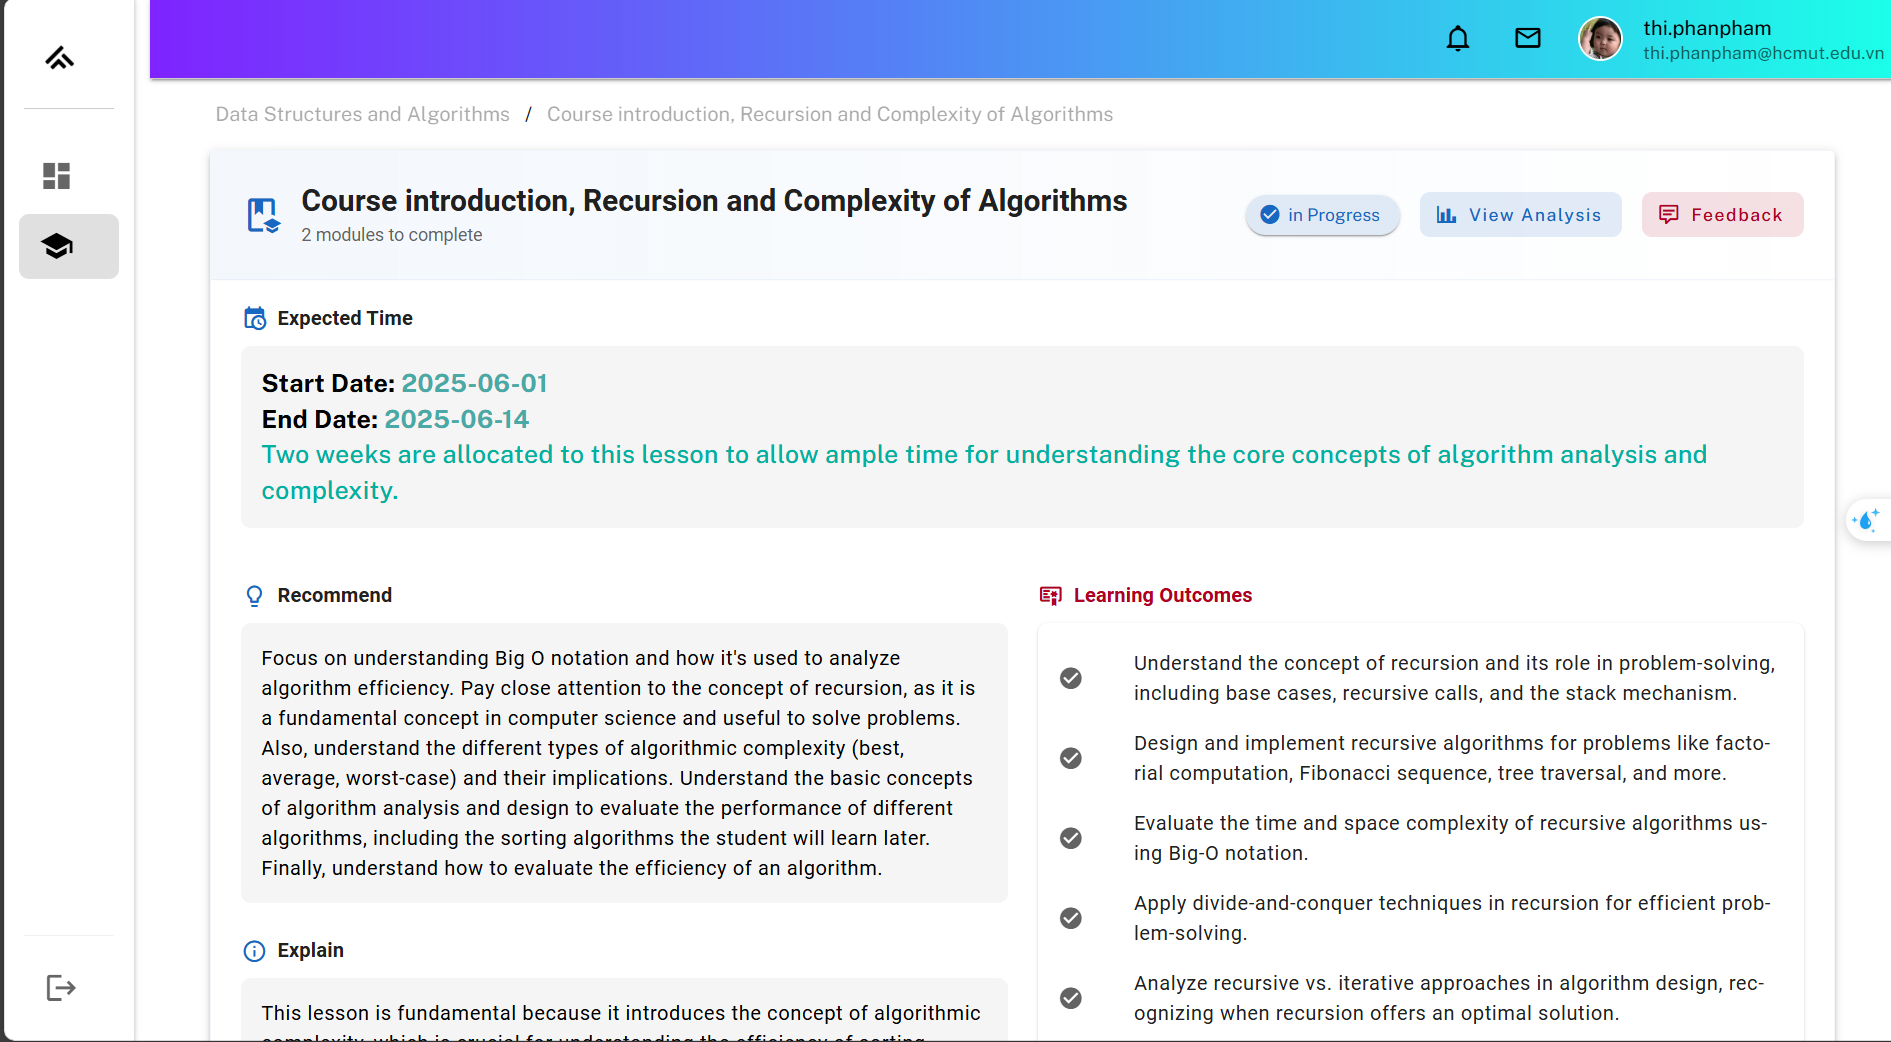
\includegraphics[width=0.8\textwidth]{images/CapScreen_Student/RecommendLessonDetail.png}
    \caption{Giao diện chi tiết bài học của sinh viên}
    \label{fig:lesson_detail_page}
\end{figure}
Giao diện chi tiết bài học được đề xuất nằm trong lộ trình học của sinh viên. Tại đây, sinh viên có thể xem thông tin chi tiết về bài học, bao gồm giải thích của AI về nội dung bài học, lý do tại sao bài học này được đề xuất và các modules học tập liên quan. Sinh viên có thể xem ngày bắt đầu và ngày kết thúc của bài học để theo dõi tiến độ học tập của mình. Các modules cần thiết cho bài học sẽ được liệt kê ở dưới cùng.

\begin{figure}[H]
    \centering
    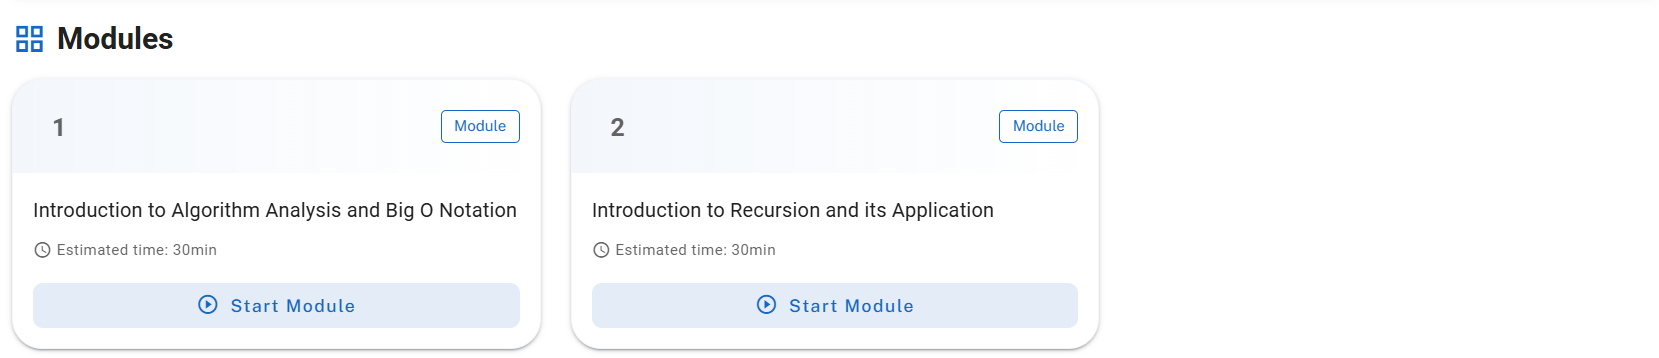
\includegraphics[width=0.8\textwidth]{images/CapScreen_Student/ViewModule.png}
    \caption{Danh sách các modules học tập của bài học}
    \label{fig:lesson_detail_page2}
\end{figure}

Ngoài ra, sinh viên có thể xem kết quả phân tích học tập của mình đối với bài học này để biết được mình có đủ kiến thức để qua bài học khác hay không hay cần ôn lại kiến thức ở bài học nào. 
\subsection{Chi tiết module}
\begin{figure}[H]
    \centering
    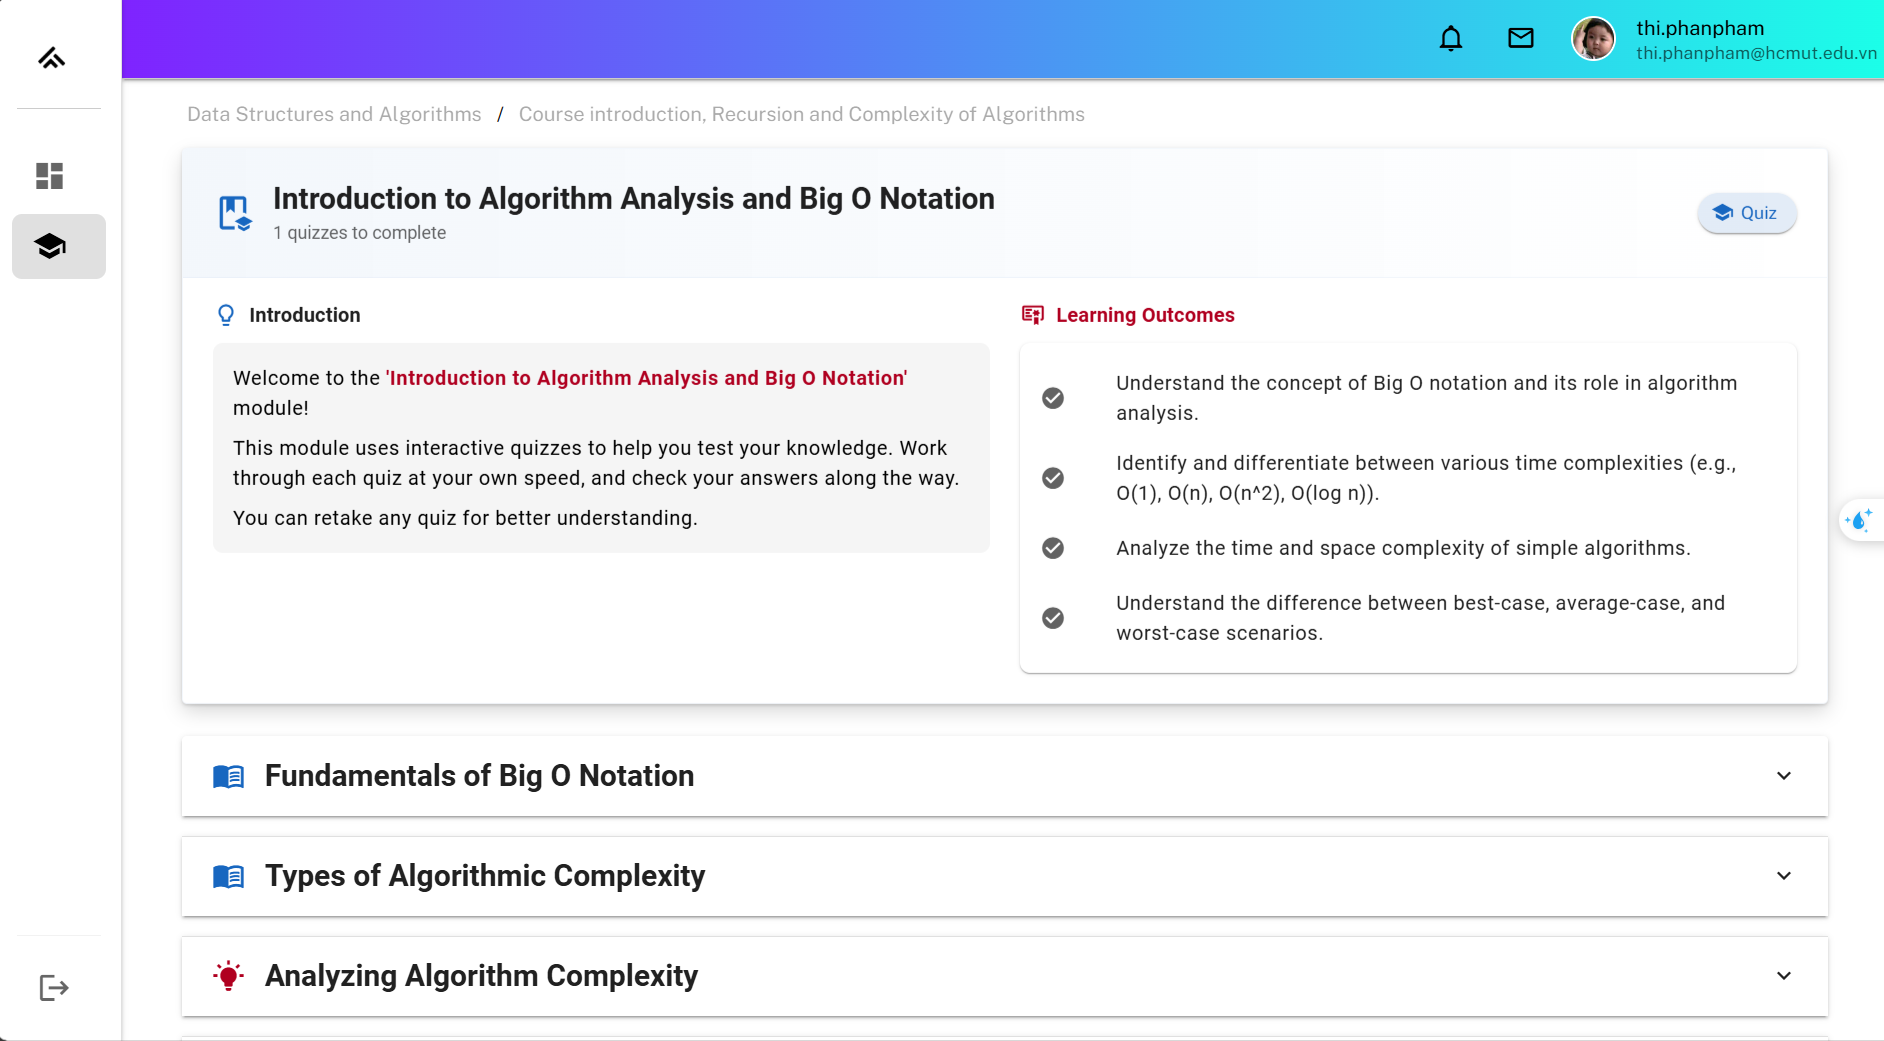
\includegraphics[width=0.8\textwidth]{images/CapScreen_Student/ModuleDetail.png}
    \caption{Giao diện chi tiết module của sinh viên}
    \label{fig:module_detail_page}
\end{figure}
Giao diện chi tiết module cho phép sinh viên xem chi tiết các kiến thức cần thiết cho bài học. Sinh viên có thể sinh ra các bài quiz tùy chọn số lượng để rèn luyện kiến thức của mình. Hệ thống sẽ tự động chấm điểm và đưa ra nhận xét cho sinh viên sau khi làm bài quiz.
\subsection{Chi tiết bài quiz}
\begin{figure}[H]
    \centering
    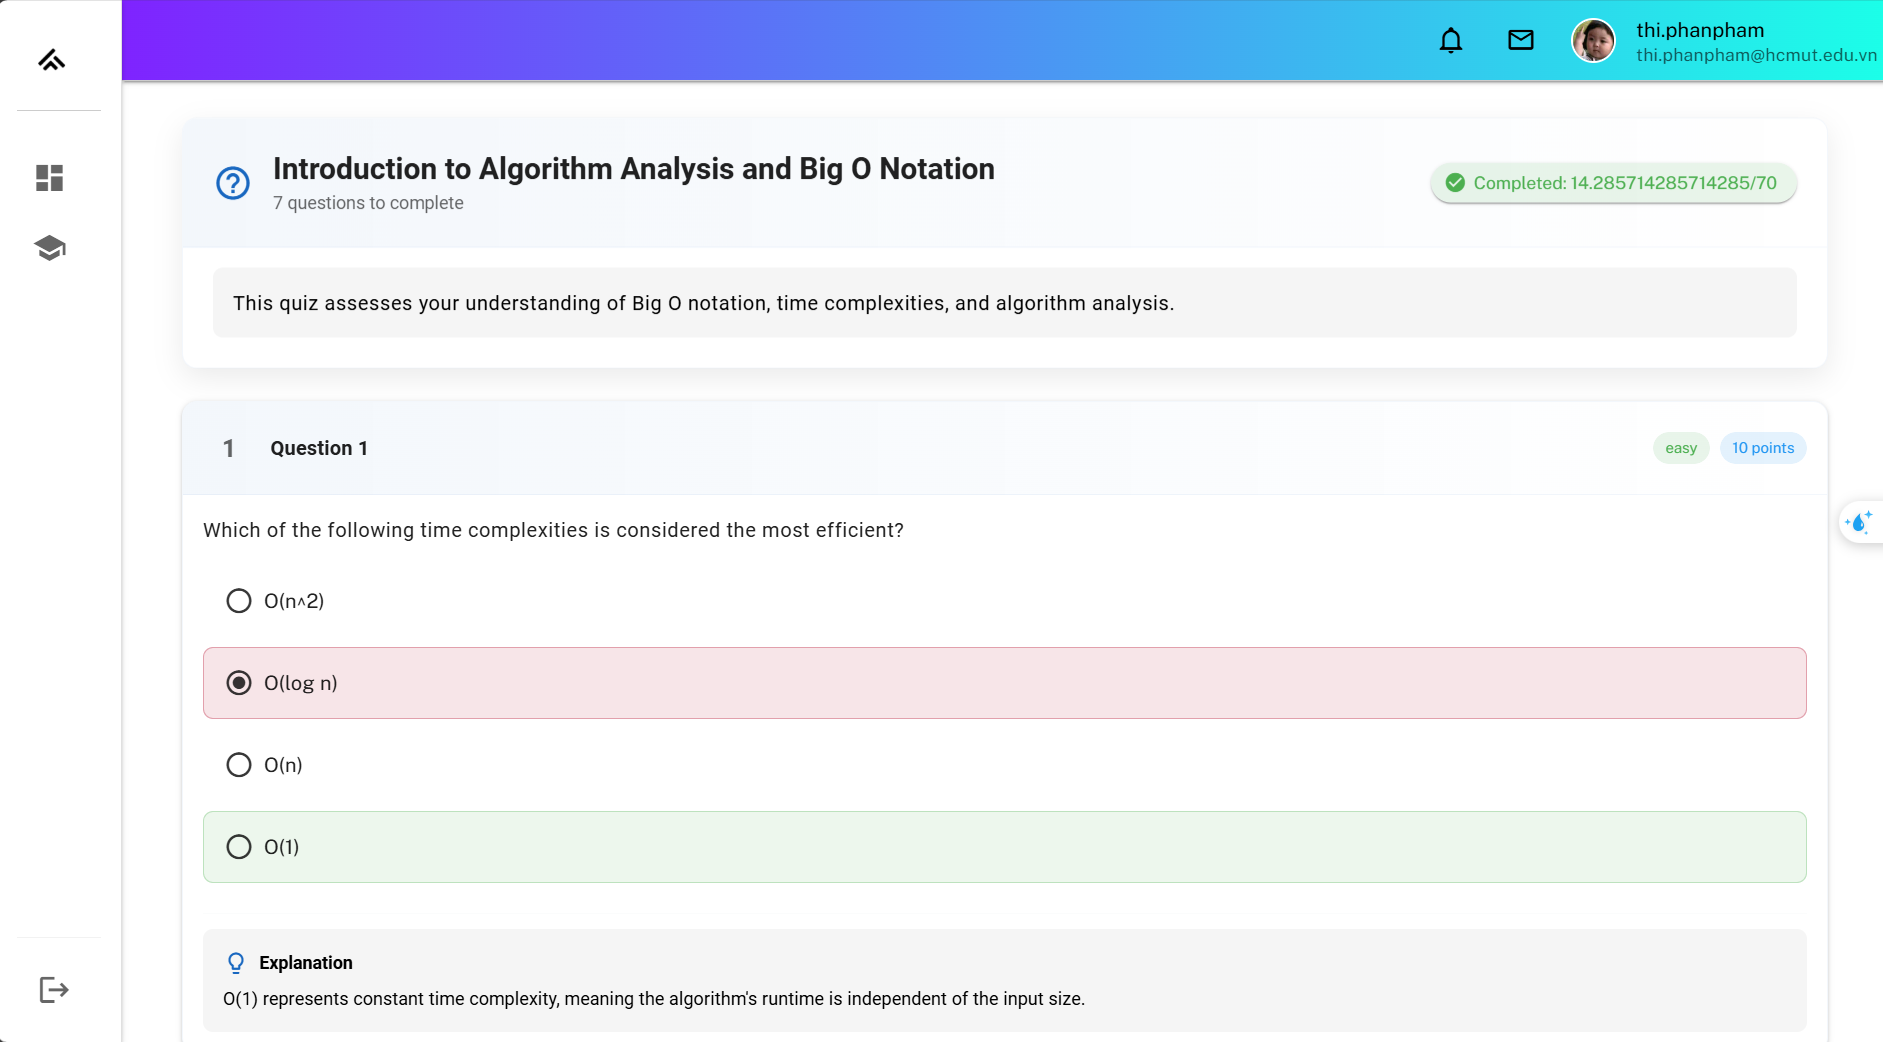
\includegraphics[width=0.8\textwidth]{images/CapScreen_Student/Quiz.png}
    \caption{Giao diện chi tiết bài quiz của sinh viên}
    \label{fig:quiz_detail_page}
\end{figure}
Giao diện chi tiết bài quiz cho phép sinh viên làm bài quiz và xem kết quả sau khi làm bài. Hệ thống sẽ tự động chấm điểm và đưa ra nhận xét cho sinh viên sau khi làm bài quiz. Sinh viên có thể làm lại bài quiz nếu chưa hài lòng với kết quả hoặc sinh ra bài quiz mới để làm. Danh sách các bài quiz được hiển thị cuối trang module
\begin{figure}[H]
    \centering
    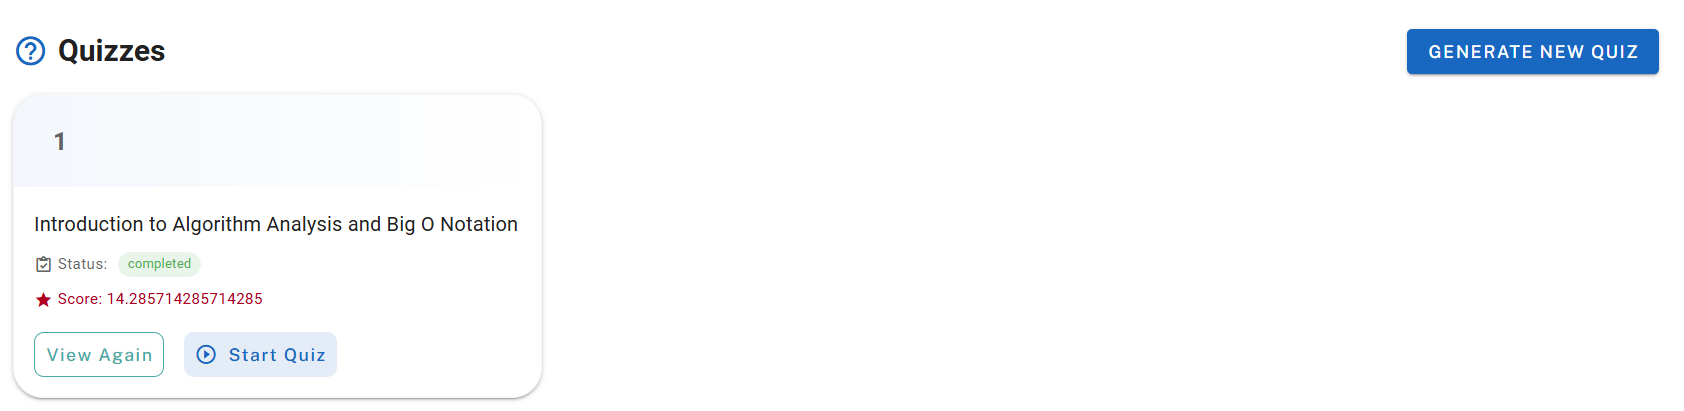
\includegraphics[width=0.8\textwidth]{images/CapScreen_Student/ViewQuiz.png}
    \caption{Danh sách các bài quiz của sinh viên}
    \label{fig:quiz_list_page}
\end{figure}
Danh sách các bài quiz cho phép sinh viên xem danh sách các bài quiz đã làm và kết quả của từng bài quiz. Sinh viên có thể xem lại các câu hỏi và đáp án của mình trong từng bài quiz.

\section{Giảng viên}
\subsection{Giao diện chính}
Trang Dashboard giáng viên cung cấp một giao diện trực quan giúp điều hướng đến những trang khác một cách dễ dàng gồm các thành phần chính như sau:
\begin{itemize}
    \item Thống kê giảng viên:
    \begin{itemize}
        \item Hiển thị tổng số khóa học mà giảng viên quản lý: chuyển đến trang danh sách khóa học
        \item Tổng số sinh viên đang theo học trong các khóa học: chuyển đến trang tiến độ sinh viên trong khóa học
        \item Hiển thị tổng số bài giảng mà giảng viên đã thiết lập.
        \item Hiển thị tổng số bài tập đã được giao cho sinh viên: chuyển đến trang tạo bài tập.
    \end{itemize}
    \begin{figure}[H]
        \centering
        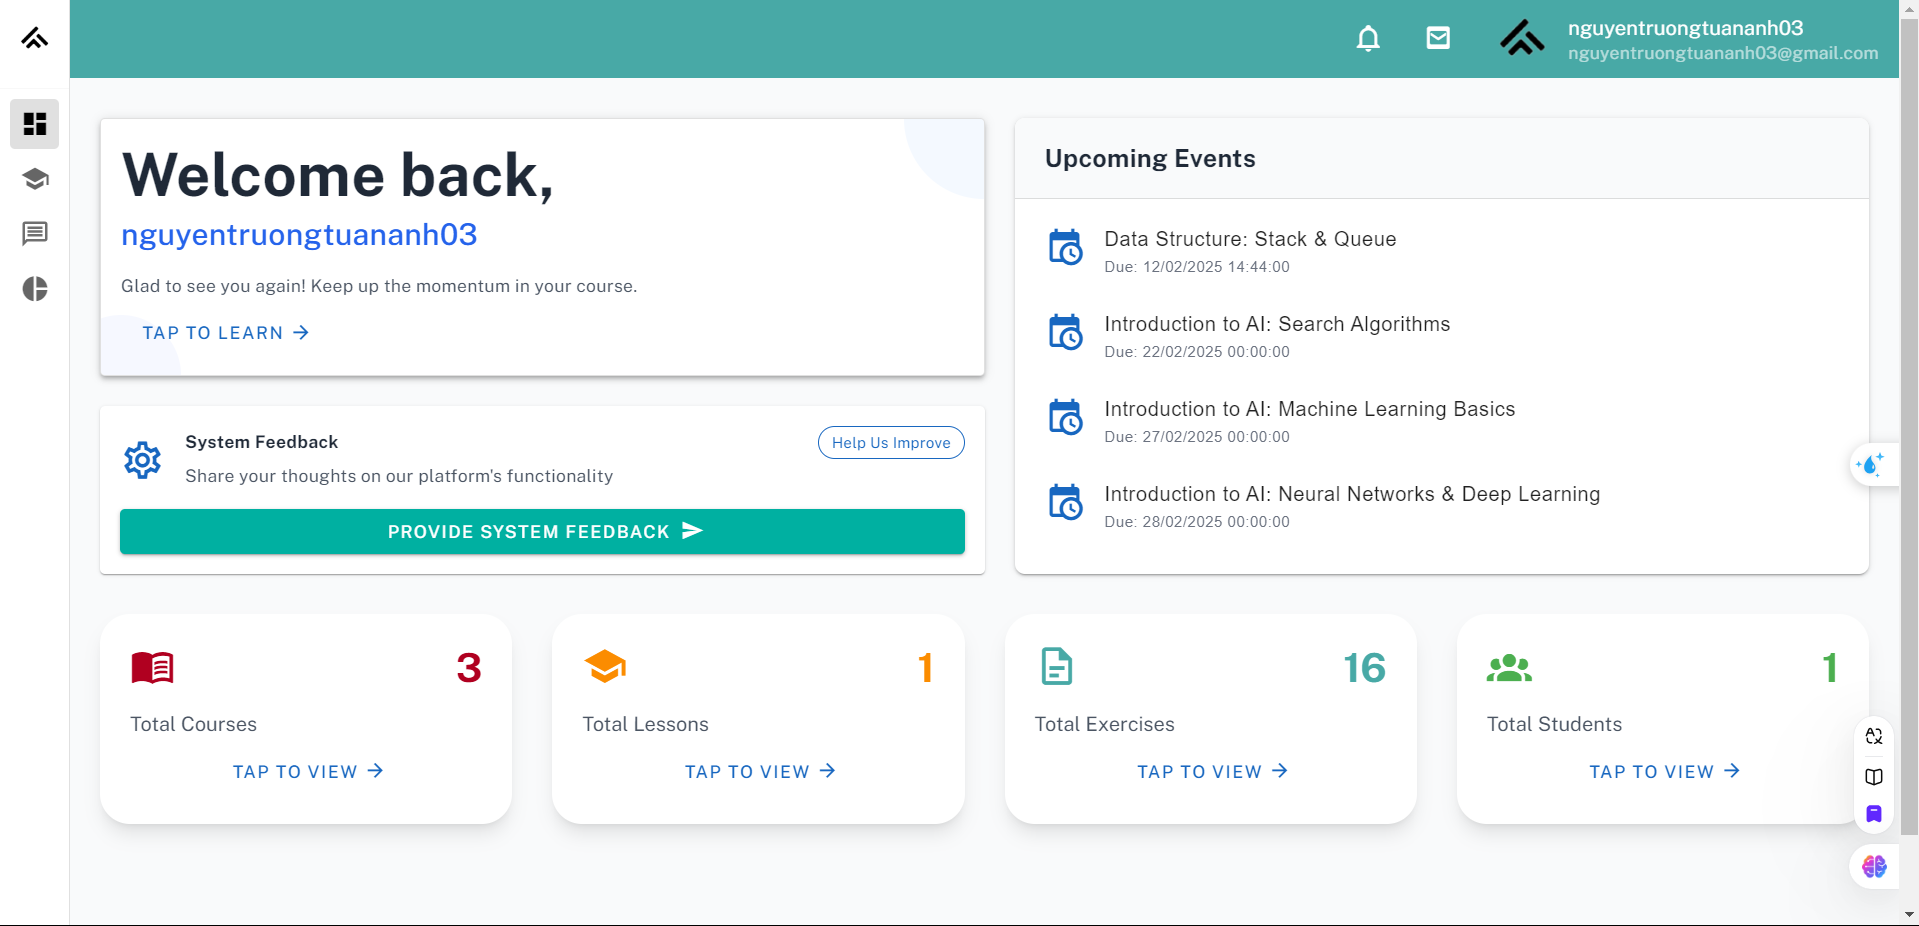
\includegraphics[width=0.8\linewidth]{images/dashboard_professor.png}
        \caption{Dashboard Professor}
        \label{fig:dashboard_professor}
    \end{figure}
    \item Upcoming Events: hiển thị danh sách các sự kiện quan trọng sắp diễn ra mà giảng viên cần quan tâm (Hạn nộp bài tập, kỳ thi, sự kiện liên quan đến học viên)
    \item Gửi Feedback cho hệ thống: Giảng viên có thể gửi feedback về hệ thống qua một modal.
    \begin{figure}[H]
        \centering
        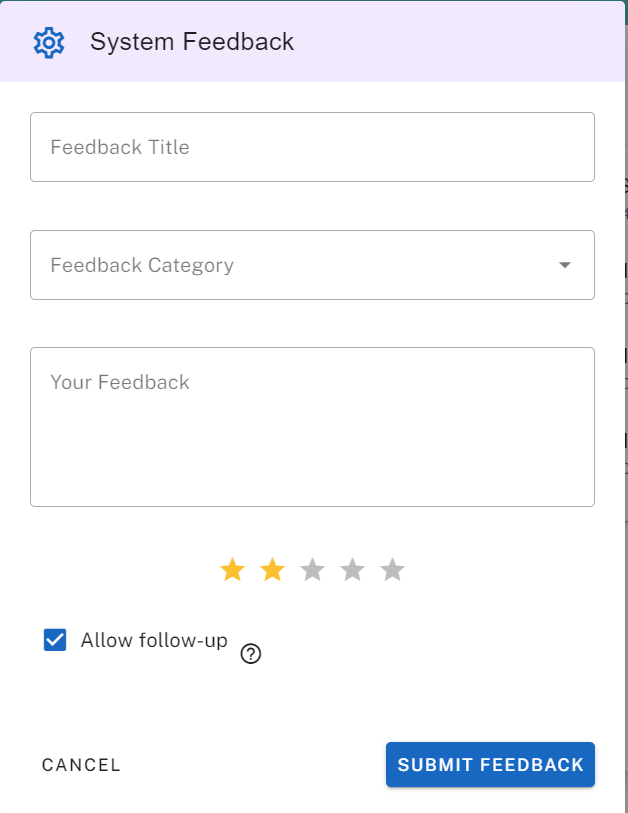
\includegraphics[width=0.3\linewidth]{images/modal_feedback.png}
        \caption{Modal Feedback}
        \label{fig:modal_feedback}
    \end{figure}
\end{itemize}
\subsection{Quản lý khóa học}
Trang My Course cung cấp danh sách các khóa học mà giảng viên phụ trách. Mỗi khóa học gồm các thông tin chi tiết như: tên khóa học, mã khóa học, sinh viên, learning outcomes, trạng thái khóa học, thời gian khóa học.
\begin{figure}[H]
        \centering
        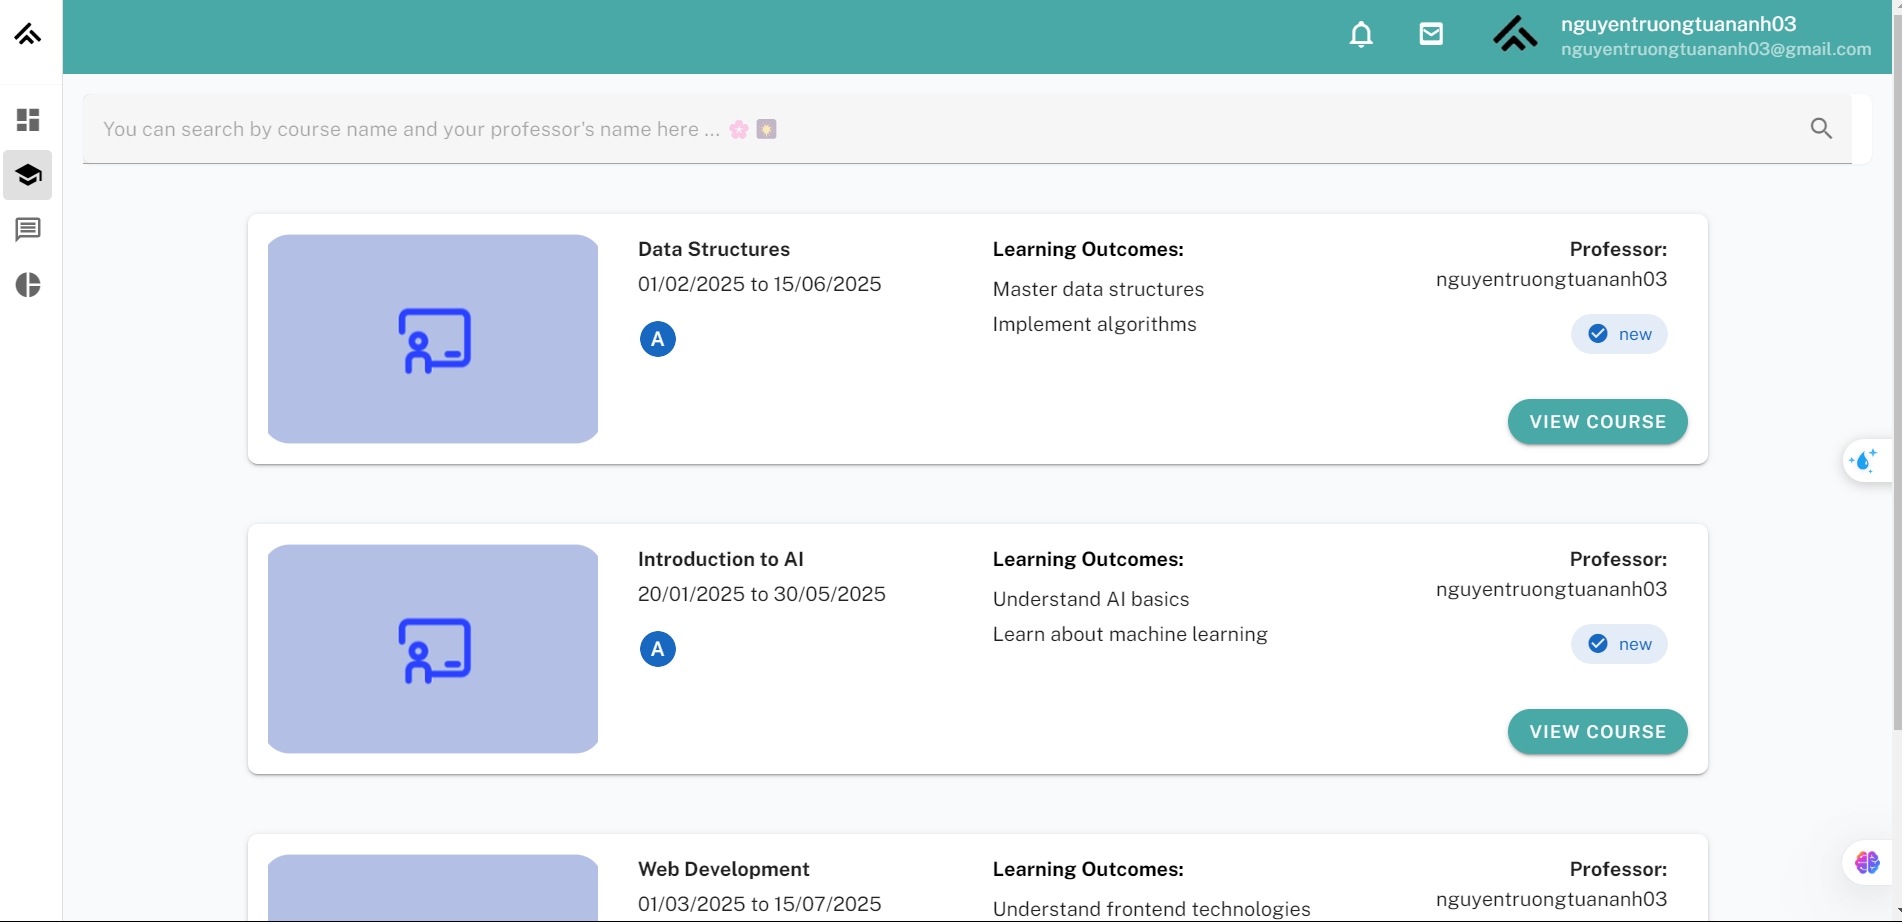
\includegraphics[width=0.8\linewidth]{images/course_professor.png}
        \caption{Professor: My Course}
        \label{fig:course_professor}
    \end{figure}
\subsection{Quản lý phản hồi của sinh viên}
Tính năng quản lý phản hồi giúp giảng viên theo dõi và phân tích ý kiến của sinh viên về khóa học.
\begin{itemize}
    \item Giảng viên có thể chọn một khóa học cụ thể từ danh sách các khóa học mà họ đang giảng dạy.
    \item Hệ thống sẽ hiển thị ra danh sách feedback gồm các thông tin: người gửi, tiêu đề phản hồi, mô tả, phân loại, rating.
    \begin{figure}[H]
        \centering
        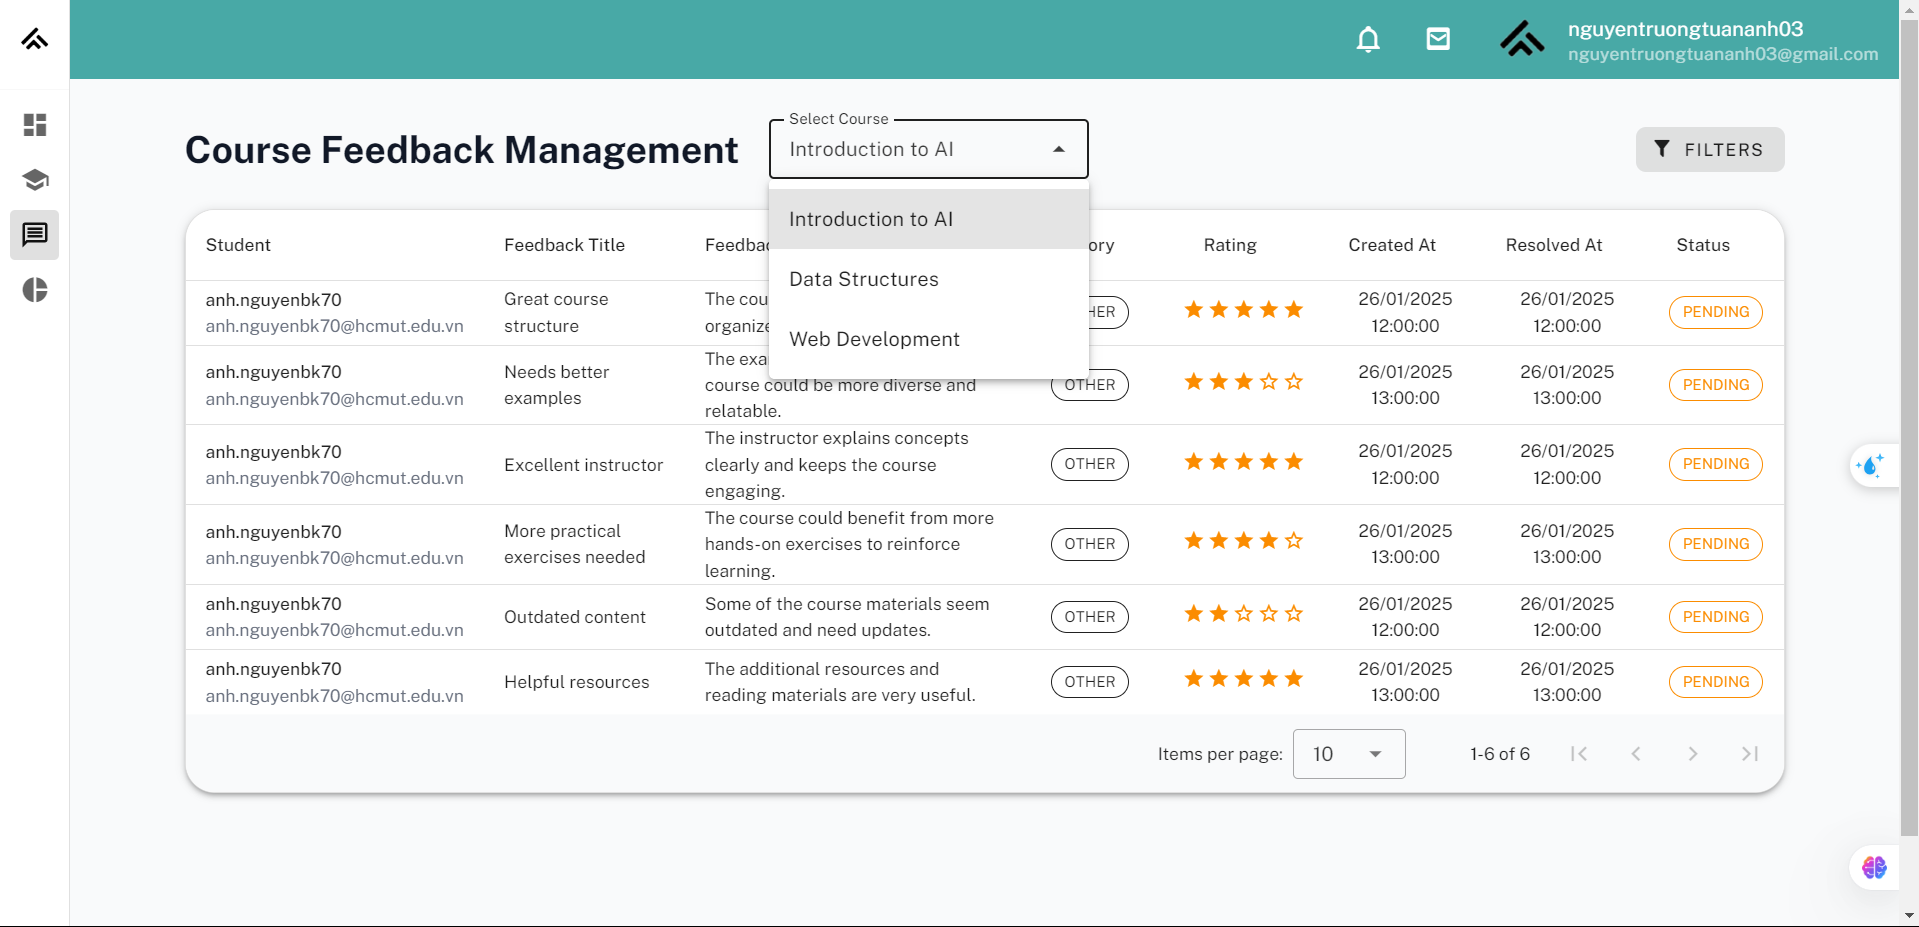
\includegraphics[width=0.8\linewidth]{images/feedback_professor.png}
        \caption{Professor: Feedback Management}
        \label{fig:feedback_professor}
    \end{figure}
\end{itemize}
\subsection{Quản lý tiến độ sinh viên}
Trang tiến độ này theo dõi tiến độ sinh viên giúp giảng viên đánh giá hiệu suất học tập của từng sinh viên trong khóa học
\begin{itemize}
    \item Tổng quan lớp học: điểm cao nhất, thấp nhất, trung bình điểm
    \item Tiến độ cá nhân: 
    \begin{itemize}
        \item Learning path cá nhân của sinh viên trong khóa học.
        \item Điểm số của từng bài kiểm tra và bài tập.
    \end{itemize}
    \item Chi tiết bài tập: Điểm của sinh viên trong bài tập, lời giải, lịch sử nộp bài và số lần thử lại.
\end{itemize}
 \begin{figure}[H]
        \centering
        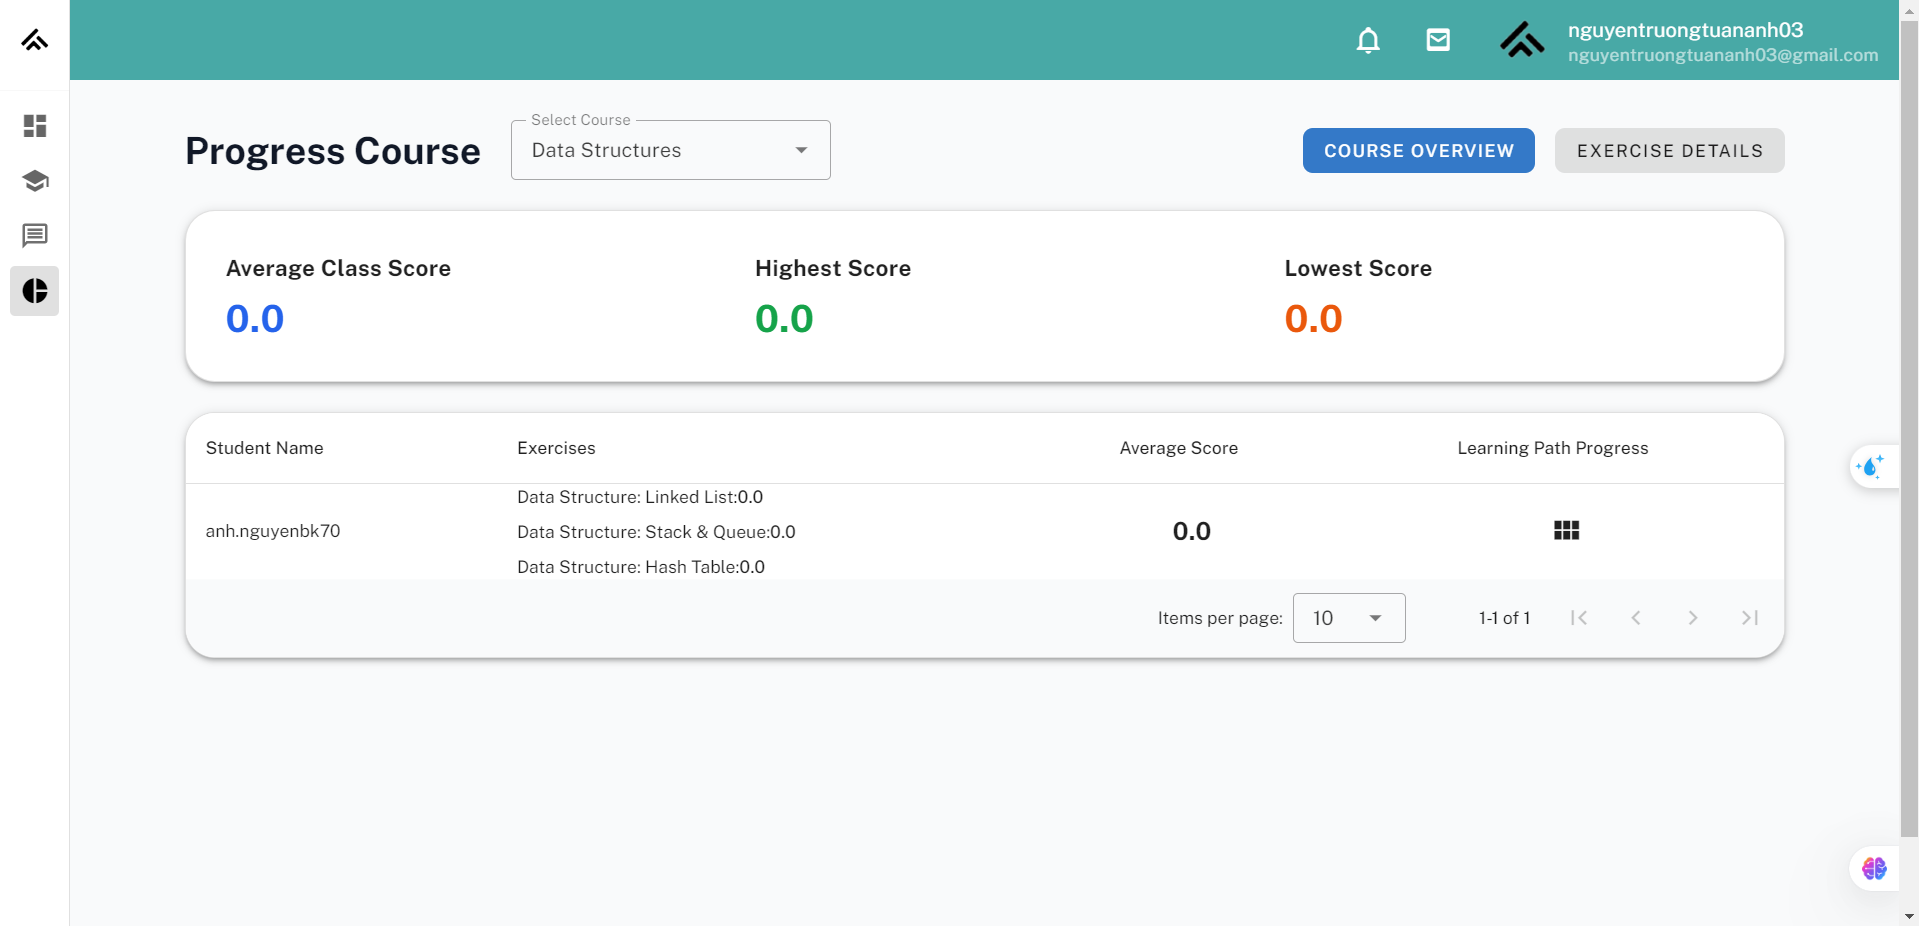
\includegraphics[width=0.8\linewidth]{images/progress_professor.png}
        \caption{Professor: Progress Student}
        \label{fig:progress_professor}
    \end{figure}
\section{Admin}
\subsection{Giao diện chính}
\begin{figure}[H]
    \centering
    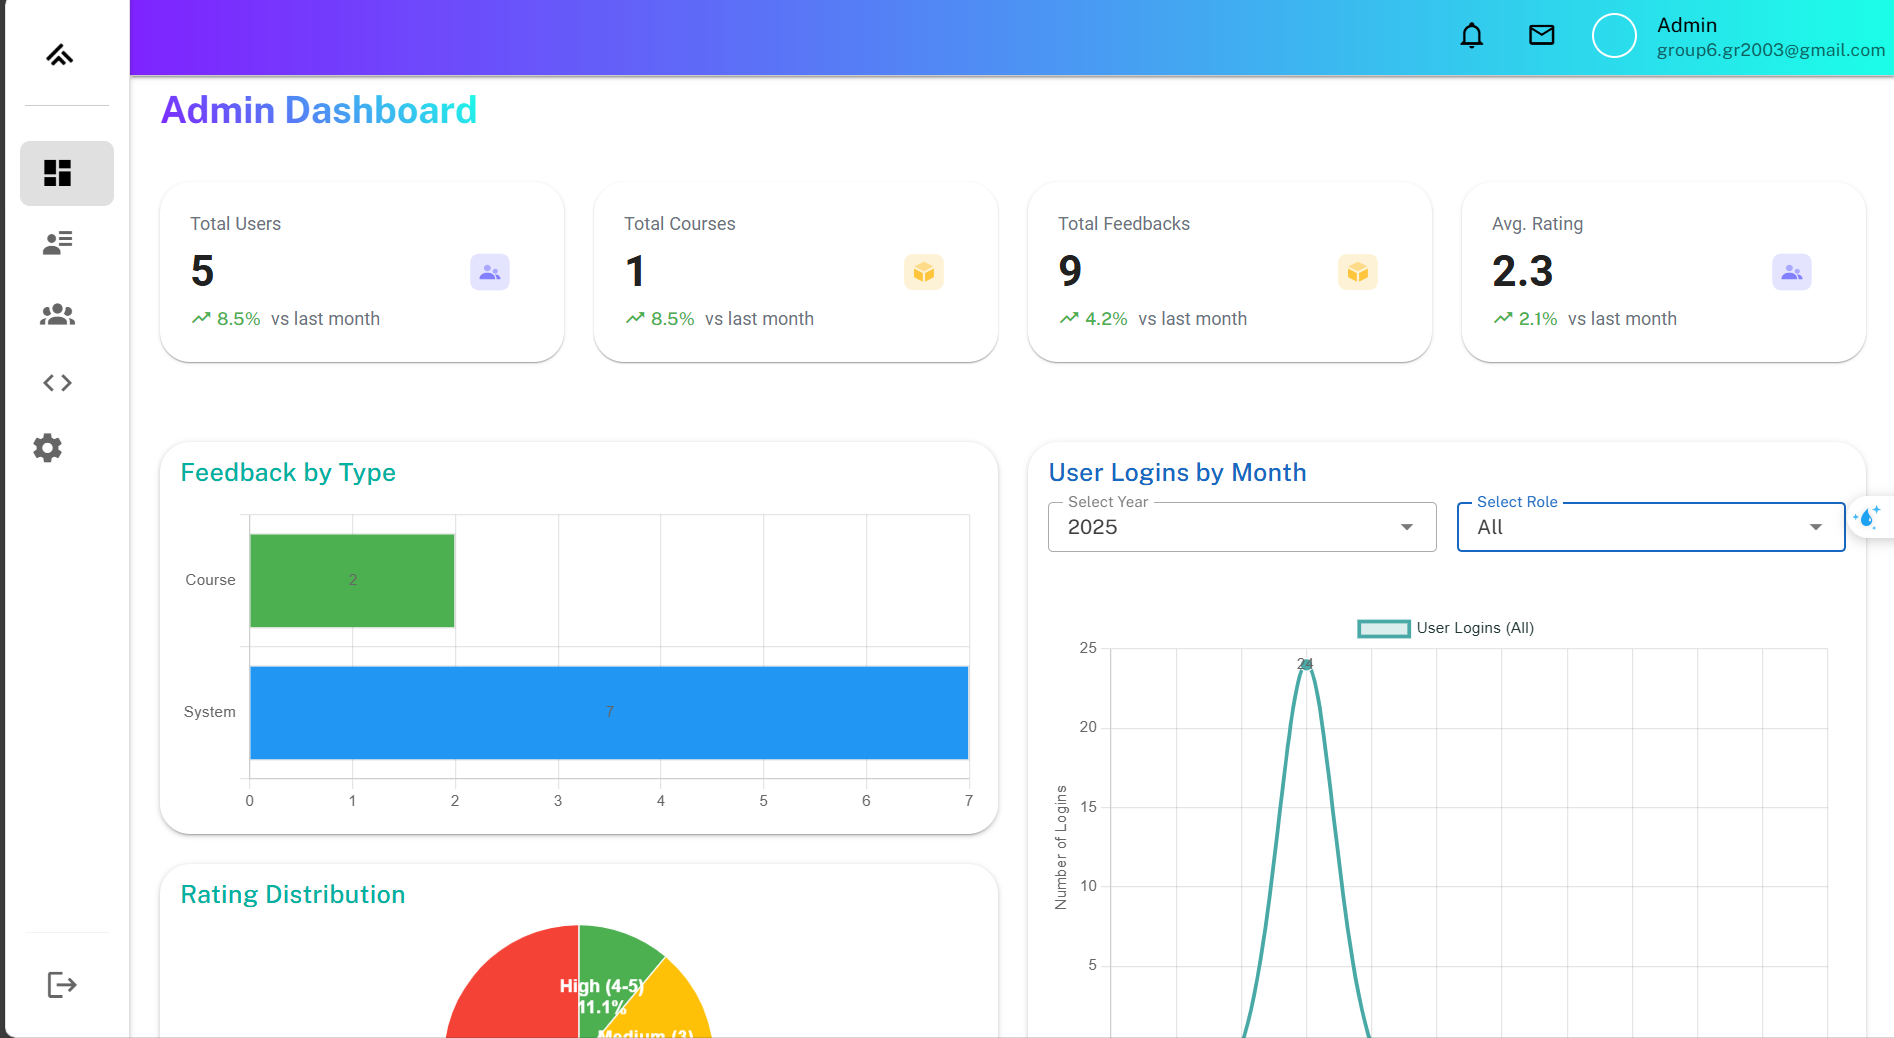
\includegraphics[width=0.8\textwidth]{images/CapScreen_Admin/dashboard.png}
    \caption{Giao diện chính của quản trị viên}
    \label{fig:admin_home_page}
\end{figure}
Giao diện chính của quản trị viên hiển thị số lượng các khóa học và người dùng trong hệ thống. Tại đây, quản trị viên có thể xem thống kê về lượng người dùng đăng nhập, thống kê về feedback của người dùng.
\subsection{Quản lý khóa học}
\begin{figure}[H]
    \centering
    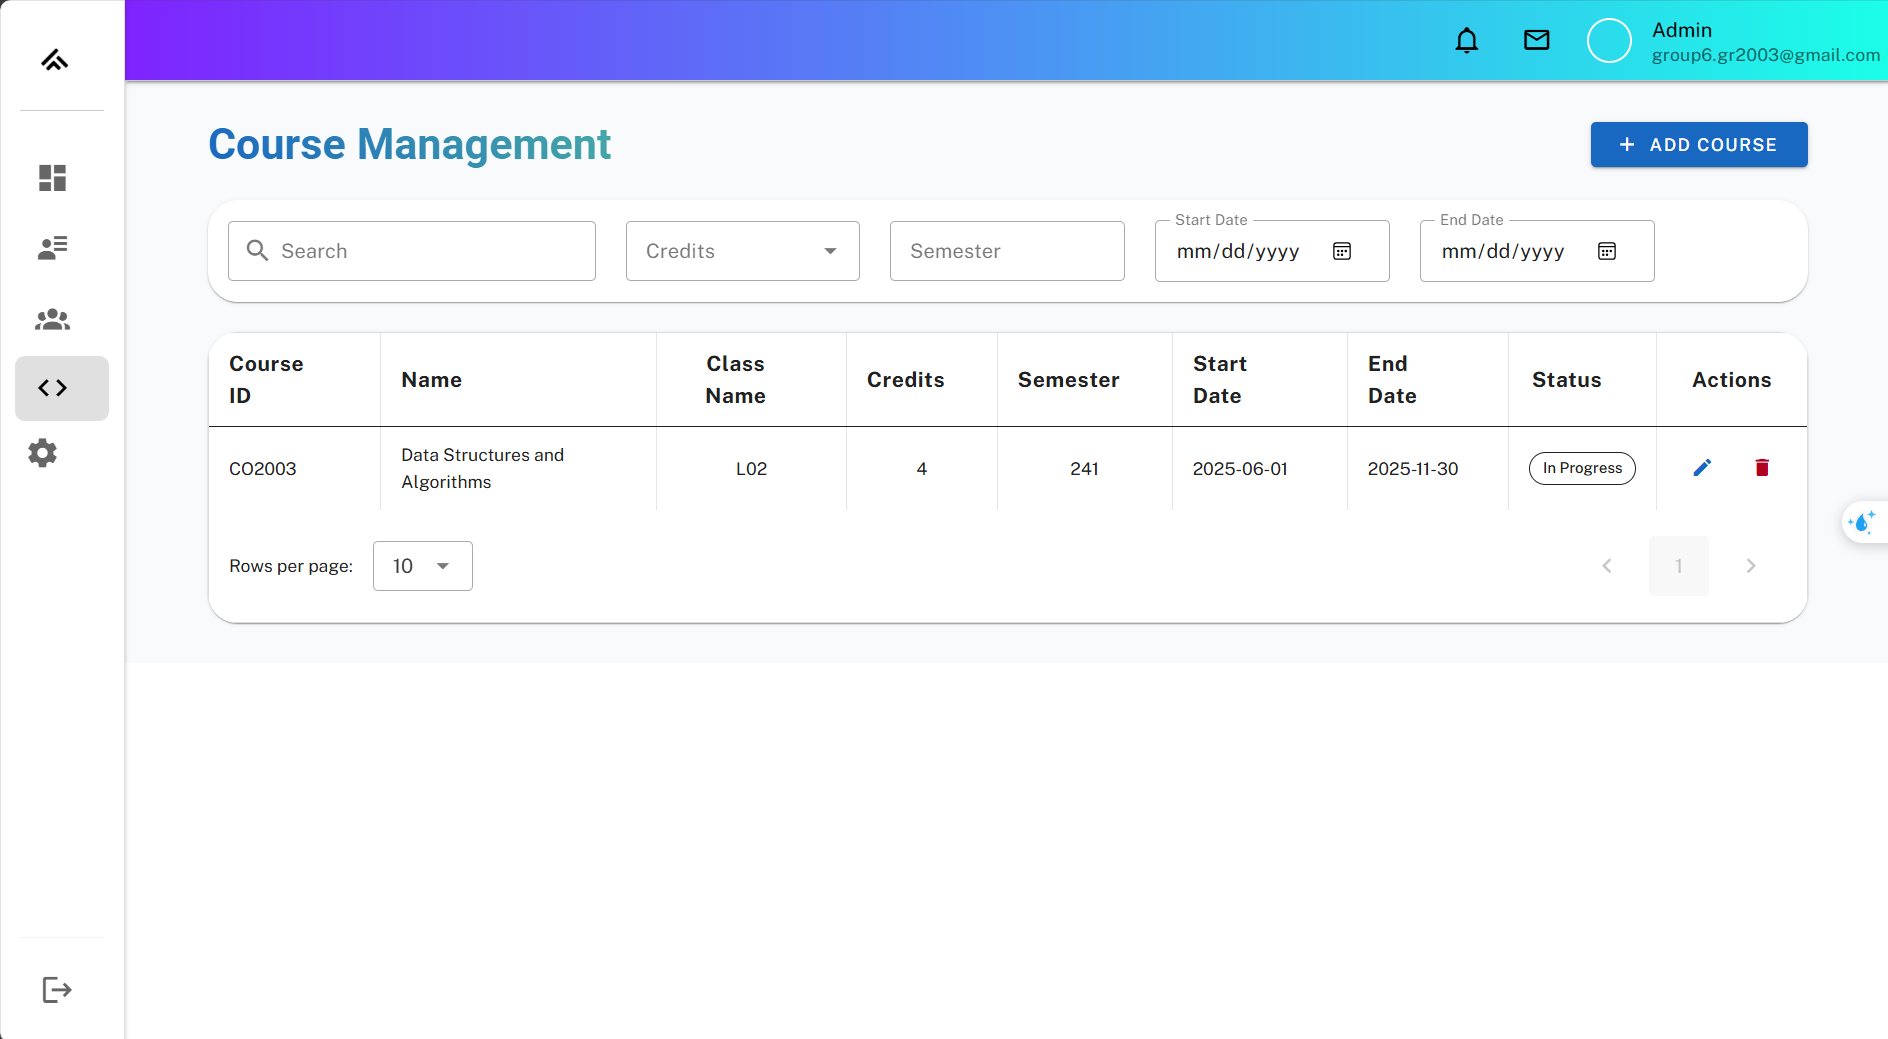
\includegraphics[width=0.8\textwidth]{images/CapScreen_Admin/course.png}
    \caption{Giao diện quản lý khóa học của quản trị viên}
    \label{fig:admin_course_page}
\end{figure}
Giao diện quản lý khóa học cho phép quản trị viên xem danh sách các khóa học trong hệ thống. Tại đây, quản trị viên có thể thêm, sửa, xóa khóa học và phân quyền cho giảng viên phụ trách khóa học.
\subsection{Quản lý người dùng}
\begin{figure}[H]
    \centering
    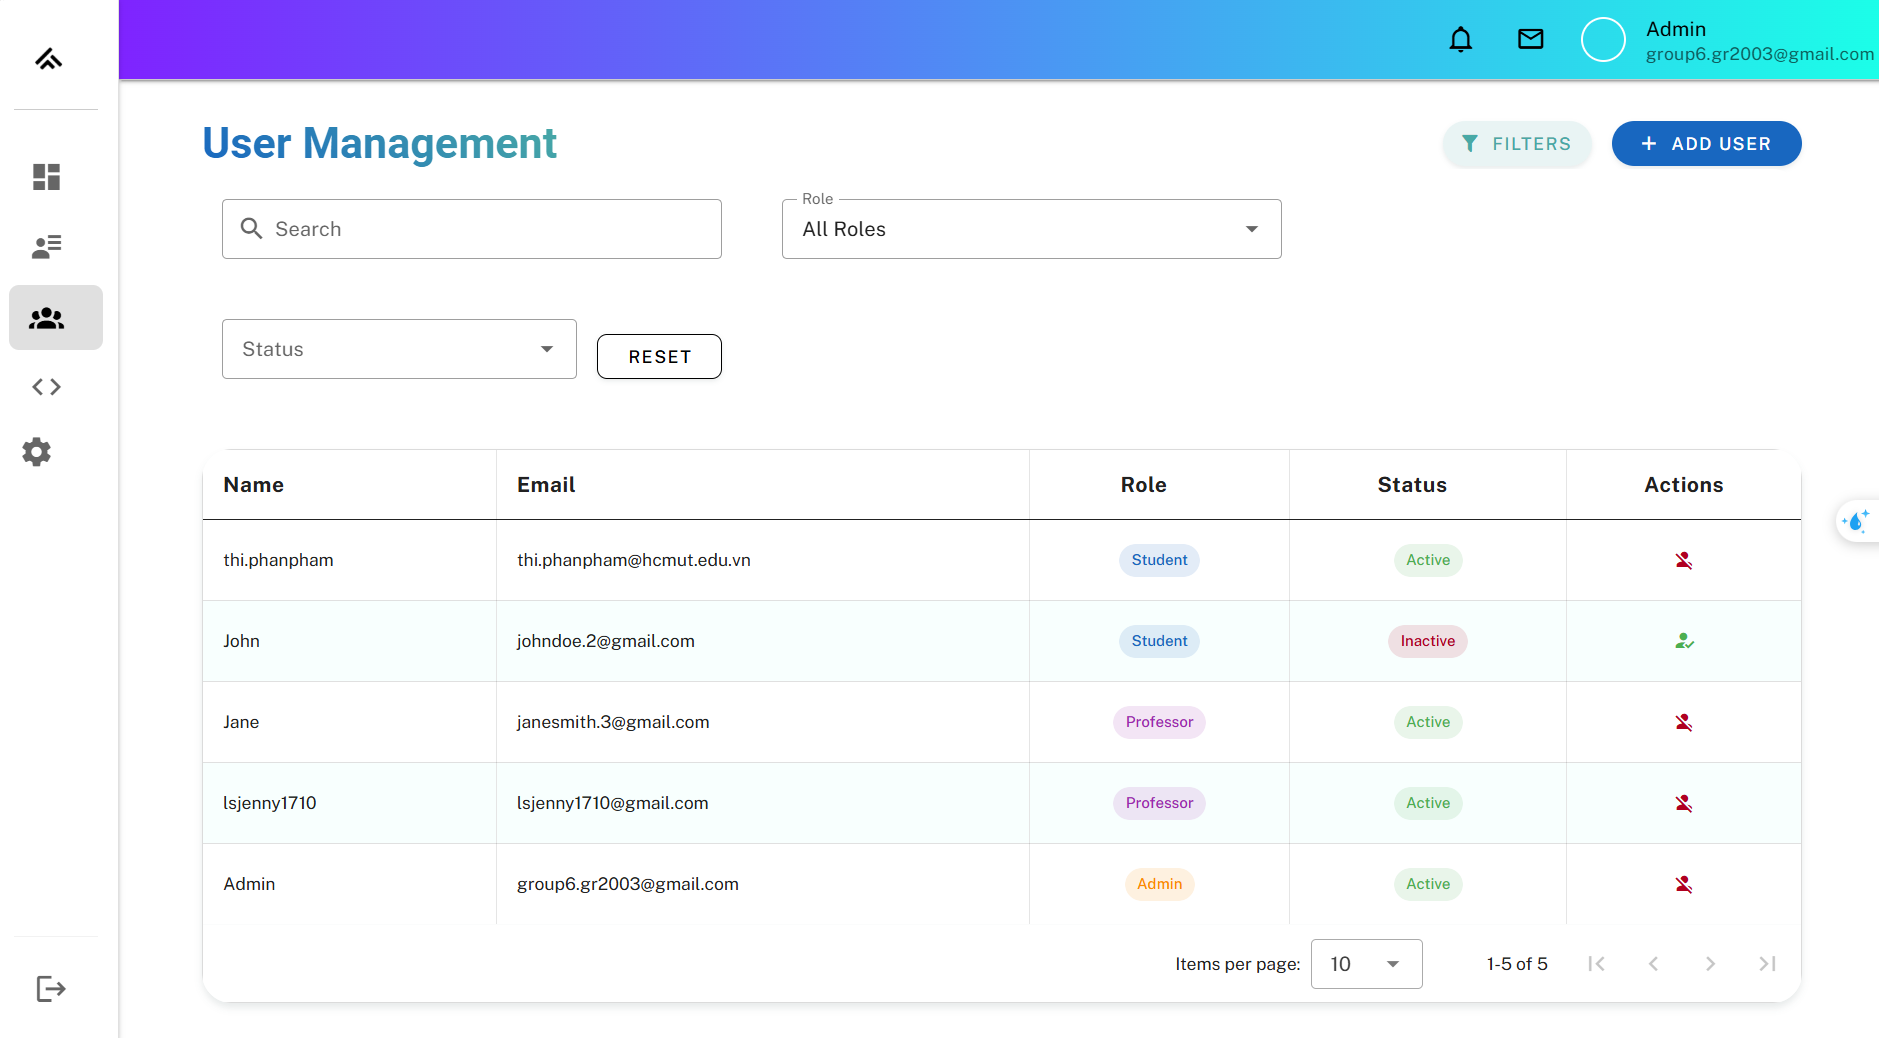
\includegraphics[width=0.8\textwidth]{images/CapScreen_Admin/user.png}
    \caption{Giao diện quản lý người dùng của quản trị viên}
    \label{fig:admin_user_page}
\end{figure}
Giao diện quản lý người dùng cho phép quản trị viên xem danh sách các người dùng trong hệ thống. Tại đây, quản trị viên có thể thêm, sửa, xóa người dùng và phân quyền cho người dùng.
\subsection{Quản lý phản hồi}
\begin{figure}[H]
    \centering
    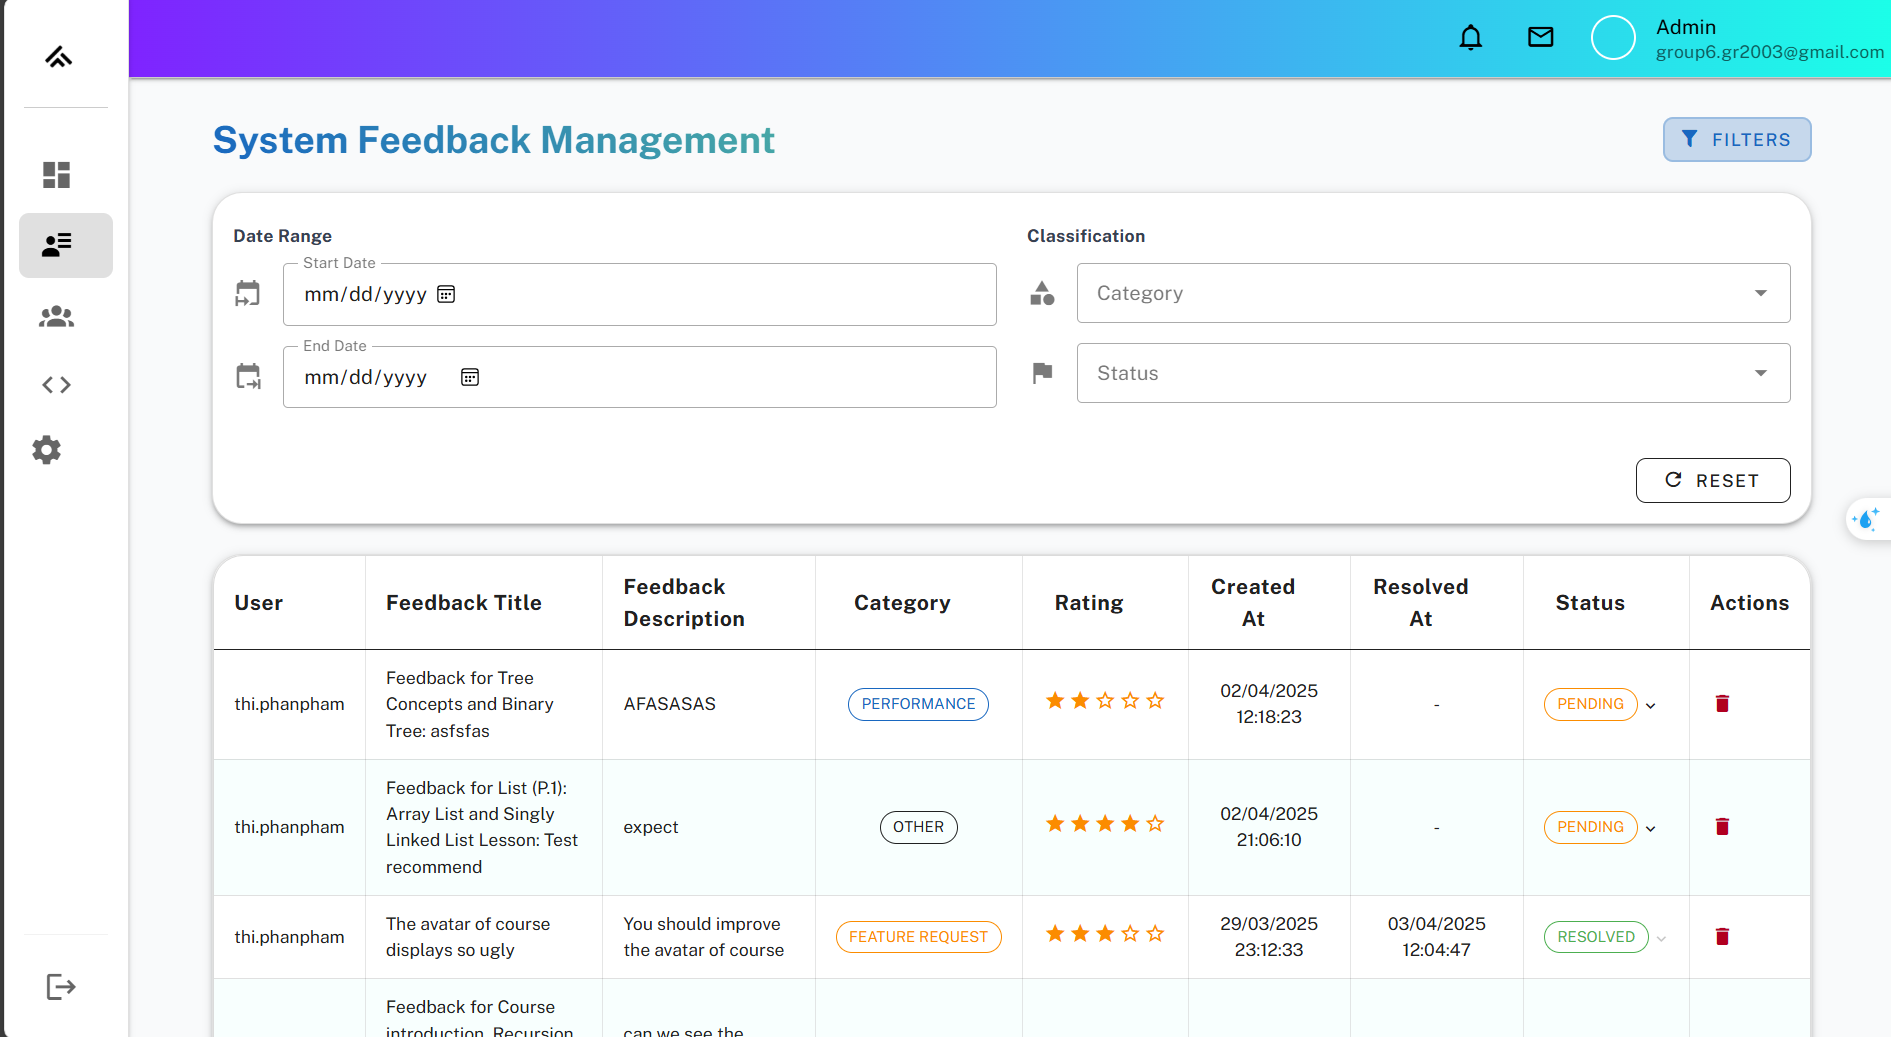
\includegraphics[width=0.8\textwidth]{images/CapScreen_Admin/feedback.png}
    \caption{Giao diện quản lý phản hồi của quản trị viên}
    \label{fig:admin_feedback_page}
\end{figure}
Giao diện quản lý phản hồi cho phép quản trị viên xem danh sách các phản hồi của người dùng trong hệ thống. Tại đây, quản trị viên có thể xem chi tiết phản hồi và trả lời phản hồi của người dùng.
\subsection{Thêm người dùng}
\begin{figure}[H]
    \centering
    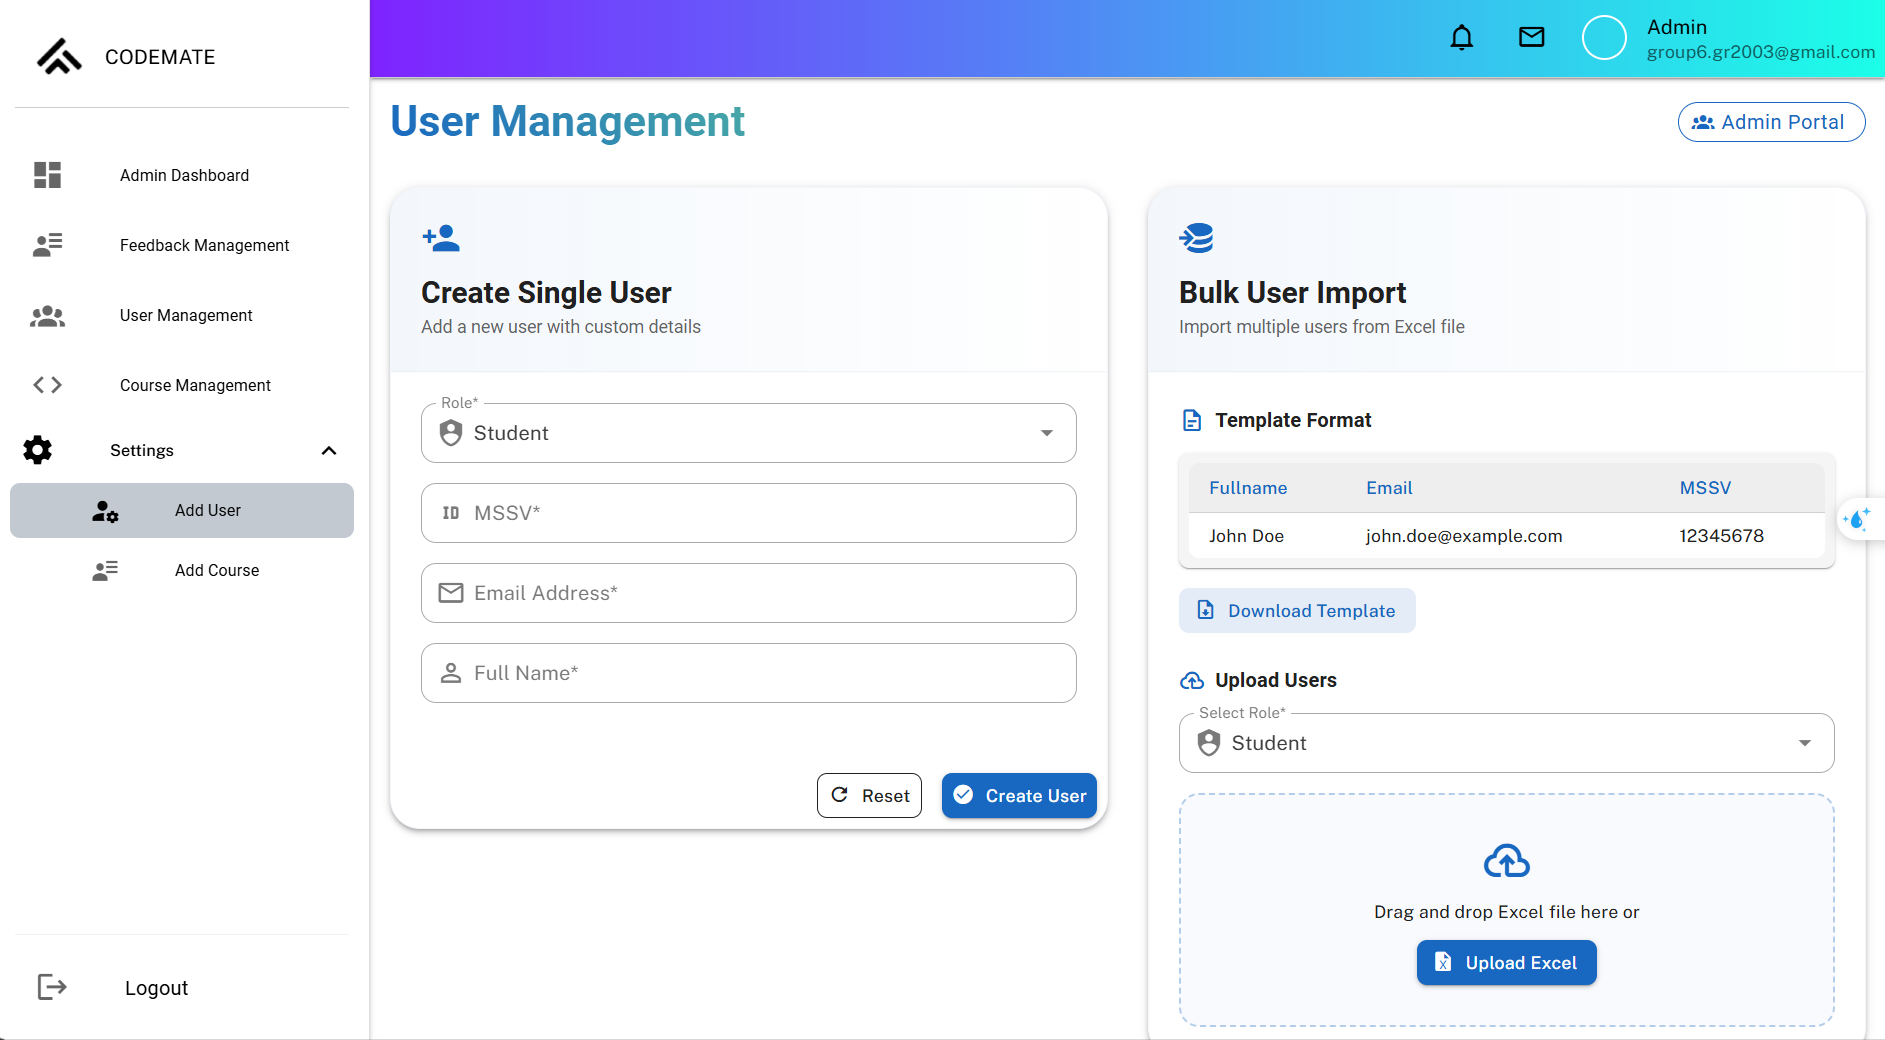
\includegraphics[width=0.8\textwidth]{images/CapScreen_Admin/adduser.png}
    \caption{Giao diện thêm người dùng của quản trị viên}
    \label{fig:admin_add_user_page}
\end{figure}
Giao diện thêm người dùng cho phép quản trị viên thêm người dùng mới vào hệ thống. Tại đây, quản trị viên có thể nhập thông tin người dùng và phân quyền cho người dùng.
\subsection{Thêm khóa học}
\begin{figure}[H]
    \centering
    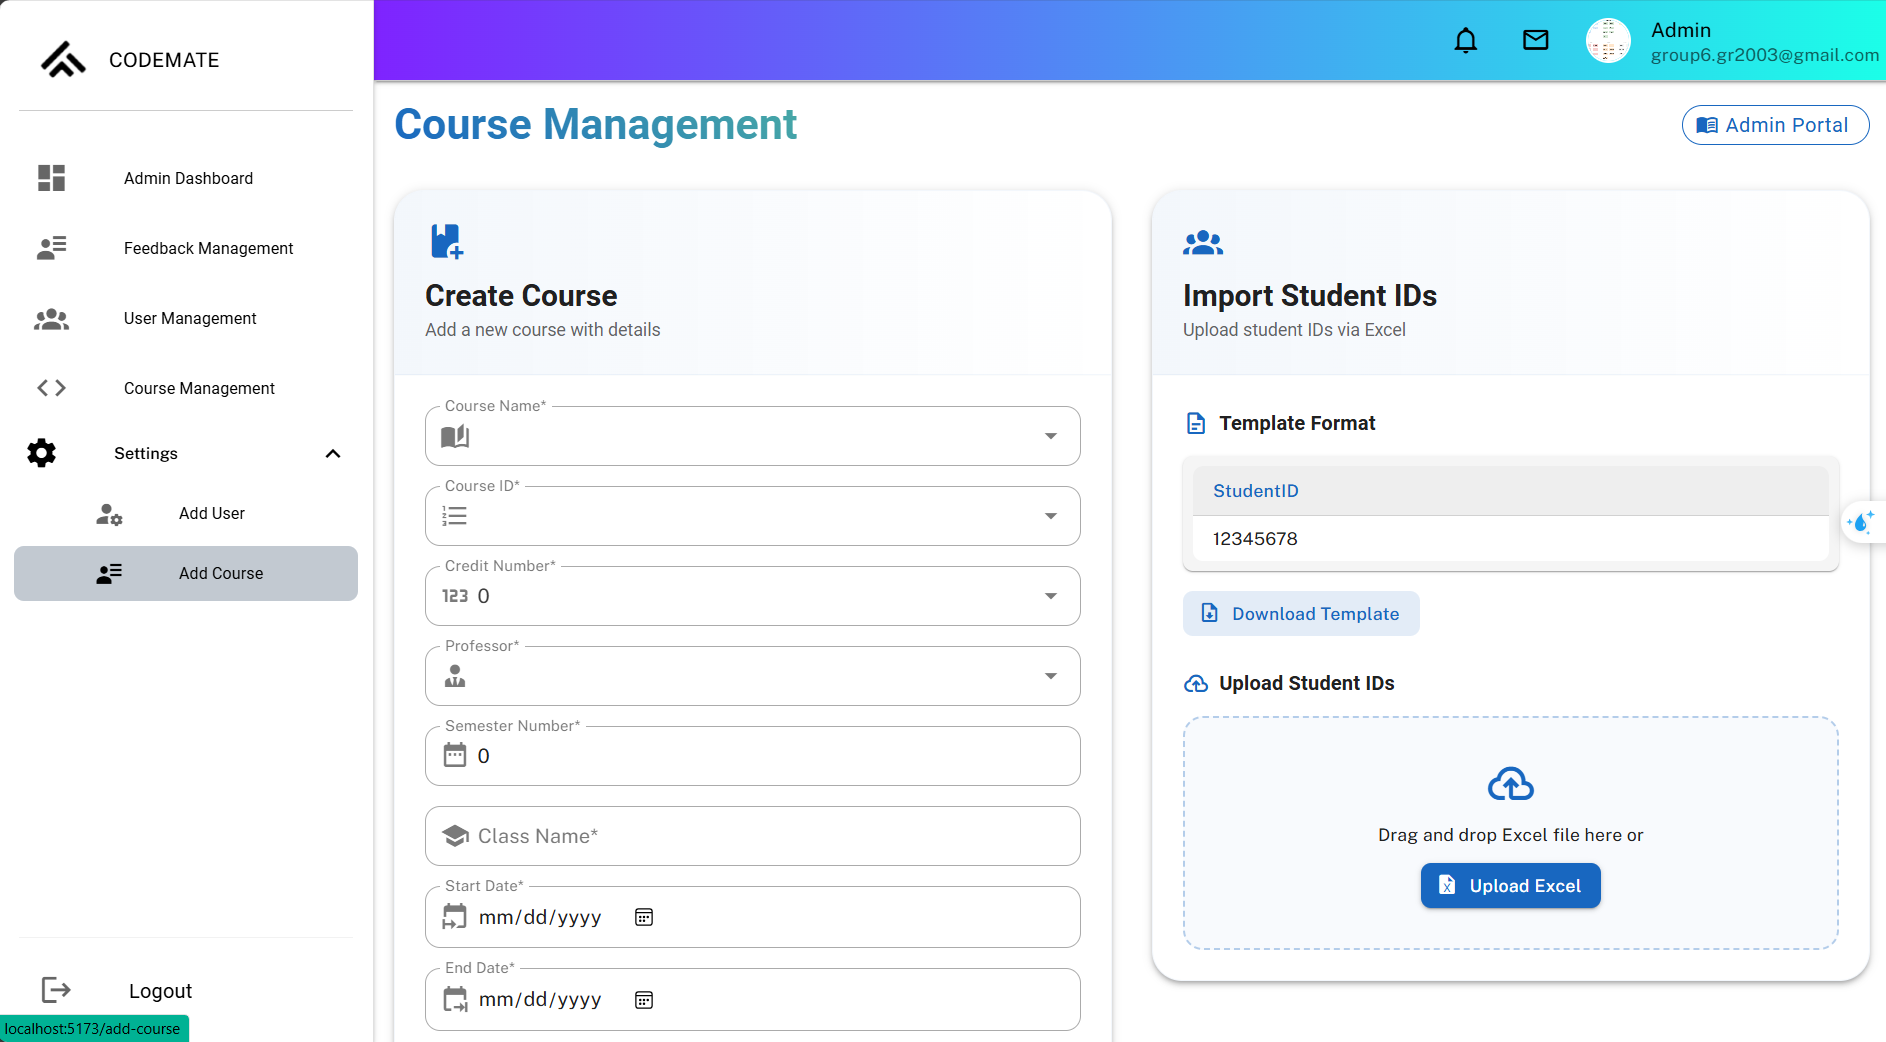
\includegraphics[width=0.8\textwidth]{images/CapScreen_Admin/addcourse.png}
    \caption{Giao diện thêm khóa học của quản trị viên}
    \label{fig:admin_add_course_page}
\end{figure}
Giao diện thêm khóa học cho phép quản trị viên thêm khóa học mới vào hệ thống. Tại đây, quản trị viên có thể nhập thông tin khóa học và phân quyền cho giảng viên phụ trách khóa học. 